%% Master thesis on Adaptive learning of programming.
\documentclass[
    %printed,
    digital,
    color,
    11pt,
    nocover,
    table,  % coloured tables; (to disable: notable)
    nolof,  % hide List of Figures
    nolot,  % hide List of Tables
    microtype,
    %final,
]{fithesis3}
%% Locales.
\usepackage[resetfonts]{cmap}
\usepackage[T1]{fontenc}
\usepackage[
  main=english,
  english, czech
]{babel}
%% Metadata.
\thesissetup{
    date          = \the\year/\the\month/\the\day,
    university    = mu,
    faculty       = fi,
    type          = mgr,
    author        = Tomáš Effenberger,
    gender        = m,
    advisor       = {doc. Mgr. Radek Pelánek, Ph.D},
    title         = {Adaptive System for Learning Programming},
    TeXtitle      = {Adaptive System for\\Learning Programming},
    keywords      = {learning programming, domain modeling, student modeling,
                     tutor modeling, programming game, adaptive learning system},
}
%% Bibliography.
\usepackage[backend=biber, 		% use biber as backend instead of BiBTeX
	%bibstyle=ieee, 	    % bibliography style: IEEE with numeric citations
	citestyle=numeric, 		    % citation style
	url=true, 			        % display urls in bibliography
	hyperref=auto,			    % detect hyperref and create links
]{biblatex}
\addbibresource{thesis.bib}
%% Abstract.
\thesislong{abstract}{%

The thesis presents an adaptive learning system for introductory programming.
To support learning and motivation, the system uses block-based programming,
a novel grid-world programming game, and progress visualisation based on
mastery learning.
By adapting difficulty of tasks to the current skills, the system helps the
students to immerse into the problem solving activity and achieve the state
of flow.
Collected data are used in offline analyses leading to insights that help
to iteratively improve the system.

%The thesis discuss strategies to support learning of introducotory programming,
% usage of artificial intelligence for adaptive behavior, design of a programming
% game, ...


%% Zadani:
%Cílem práce je vytvořit adaptabilní webový systém sloužící k výuce základů
%programování. Základní prostředí bude typu "robot pohybující se v mřížce",
%přičemž toto tradiční pojetí bude ztvárněno inovativním způsobem. Systém se
%bude přizpůsobovat dovednostem studentů předkládáním úloh vhodné obtížnosti a
%bude tak maximalizovat jejich čas strávený ve stavu flow. Práce bude řešit
%návrh vhodného výukového prostředí, návrh metod adaptabilního chování i
%praktickou implementaci systému. Součástí práce bude i analýza dat z provozu
%systému a vyhodnocení použitých zadání.


}
%% Thanks.
\thesislong{thanks}{%

My journey towards this thesis started 9 years ago at K-SCUK,
a week-long interdisciplinary camp for
high school students, organized by inspiring instructors.
Three of them significantly contributed to my research interests
and skills.
Jan Rygl showed me the power of artificial intelligence
% by guiding me through a project about minimax algorithm for tic-tac-toe.
and later became supervisor of my bachelor thesis.
%Many years after the camp, he supervised my bachelor thesis about automatic question generation.
Jan Papoušek became my colleage in Adaptive Learning group
and helped me to overcome many challenges involved in
the development of an adaptive learning system.
Finally, Radek Pelánek invited me to the Adaptive Learning group,
became my Master Yoda during my master studies,
gave me a lot of actionable feedback,
and never hesitated to dive with me into a fruitful brainstorming.

Several other friends contributed to the
development of the adaptive learning system described in this thesis;
by implementing some of its parts, performing analyses, discussing ideas,
creating illustrations for the web, %discussing programming issues,
or by helping me with deployment of the system:
Jaroslav Čechák, Jiří Mauritz, Jiří Řihák, Matěj Vaněk, and Barbora Vrzáková.
I am also grateful to all people who tried the system
and gave me a feedback.

\bigskip
The development of the adaptive learning system was supported by Red Hat
and Masaryk University Rector Project for outstanding master theses.
}
%% Index.
\usepackage{makeidx}      %% The `makeidx` package contains
\makeindex                %% helper commands for index typesetting.
%% Compact lists.
\usepackage{paralist}
\usepackage{enumitem}
\setitemize{noitemsep,topsep=3pt,parsep=3pt,partopsep=3pt}
%% Mathematics
\usepackage{amsmath}
\usepackage{amsthm}
\usepackage{amsfonts}
\usepackage{amssymb}
%% Graphics
\usepackage{tikz}
%% Colors
\usepackage{xcolor}
\definecolor{theme-red}{rgb}{0.62,0.01,0.05}
\definecolor{dark-red}{rgb}{0.6,0.15,0.15}
\definecolor{dark-green}{rgb}{0.15,0.4,0.15}
\definecolor{medium-blue}{rgb}{0,0,0.5}
\definecolor{light-gray}{rgb}{0.93,0.93,0.93}
\definecolor{gray}{rgb}{0.5,0.5,0.5}
%% Source code highlighting
\usepackage{listings}
\lstset{
  backgroundcolor=\color{light-gray},
  frame=lines,
  rulecolor=\color{black},
  numbers=left,
  numberstyle=\tiny\color{gray},
  basicstyle=\ttfamily,
  showspaces=false,
  showstringspaces=false,
  escapeinside={<*}{*>},
  belowskip=0.2em,
  %identifierstyle=\color{black},
  %keywordstyle=\color{blue},
  %stringstyle=\color{teal},
  commentstyle=\itshape}
%% Subcaption package for subfigure environment.
\usepackage{subcaption}
\captionsetup[subfigure]{
  width=0.97\textwidth,
  justification=raggedright,
}
%% URLs.
\usepackage{url}
\usepackage{hyperref}
%% References.
\usepackage[capitalise,noabbrev]{cleveref}  % Must be loaded after hyperref.
%% Include shared macros used across chapters.
%--------------------------------------------------------------------
% Page-wide centered image with caption.
%--------------------------------------------------------------------
% #1: proportion of textwidth to use [optional, default: 1]
% #2: image ID
% #3: caption
\newcommand{\imgW}[3][1] {
\begin{figure}[htb]
\centering
\includegraphics[width=#1\textwidth]{img/#2}
\caption{#3}
\label{fig:#2}
\end{figure}
}


% Image with caption endign with a footnote.
% TODO: Make sure that footnote is on the same page as the figure.
\newcommand{\imgWithFootnote}[4][1] {
\begin{figure}[h]
  \begin{center}
    \includegraphics[width=#1\textwidth]{img/#2}
  \end{center}
  \caption[#2]{#3\protect\footnotemark}
  \label{fig:#2}
\end{figure}
\footnotetext{#4}
}


%--------------------------------------------------------------------
% Splitting listings into "from" and "to" part
%--------------------------------------------------------------------
\newcommand{\arrowlinesplit}{%
  \noindent\makebox[\linewidth]{\raisebox{0.15em}{\rule{0.450\textwidth}{0.5pt}}%
  ~$\downarrow$~%
  \noindent\raisebox{0.15em}{\rule{0.450\textwidth}{0.5pt}}}%
}

%--------------------------------------------------------------------
% Quotes with italics.
%--------------------------------------------------------------------
%\newenvironment{itquote}
%{\begin{quote}\itshape}
%{\end{quote}}

\newenvironment{widequote}[1]%
  {\list{}{\leftmargin=#1\rightmargin=#1}\item[]}%
  {\endlist}

\newcommand{\itquote}[3][10mm] {
\begin{widequote}{#1}
\emph{#2} (#3)
%--- #3
\end{widequote}
}

\newcommand{\itquoteright}[3][10mm] {
\begin{widequote}{#1}
\emph{#2}
\vspace{-4.5mm}
\begin{flushright}
(#3)
\end{flushright}
\end{widequote}
}


%--------------------------------------------------------------------
% Definition of JavaScript listing
% Source: https://tex.stackexchange.com/questions/89574/language-option-supported-in-listings
% Usage: \begin{lstlisting}[language=ES6] ...
%--------------------------------------------------------------------
\lstdefinelanguage{ES6}{
  keywords={%
    typeof, new, true, false, try, catch, function, return, null, %
    catch, switch, var, let, const, if, in, while, do, else, case, break, yield},
  ndkeywords={class, export, boolean, throw, implements, import, this},
  sensitive=false,
  comment=[l]{//},
  morecomment=[s]{/*}{*/},
  morestring=[b]',
  morestring=[b]"
}


%--------------------------------------------------------------------
% Hyphenation setting
%--------------------------------------------------------------------
\hyphenation{analy-sis}
\hyphenation{analy-ses}


% Load fithesis prematuraly to allow custom changes.
\thesisload
%% Limit depth in Table of Contents.
\setcounter{tocdepth}{1}
% Shrink space between figure and caption
%\setlength{\abovecaptionskip}{3pt plus 3pt minus 2pt}

\begin{document}

\chapter{Introduction}
\label{chap:introduction}

Artificial intelligence is a powerful tool for tackling difficult problems,
from playing chess to driving autonomous cars.
This thesis explores how we can use artificial intelligence to optimize
learning of introductory programming.
%This thesis explores how can be artificial intelligence used to optimize
%learning of introductory programming.

Adaptive learning systems have been already successfully used in many domains
\cite{alg.evaluation-geography} (+CITE).
However, the most popular introductory programming tutorials
(Hour of Code) still use a fixed sequence of tasks for everybody,
leading to a suboptimal experience.
Aritificial intelligence can be used to personalize the sequence of tasks
for each student.
By giving students tasks of optimal difficulty, neither too easy, nor too
difficult, we help them to achieve complete immersion into the problem solving
activity, which is known as a \emph{state of flow} \cite{flow}
(figure \ref{fig:flow}).
The state of flow is essential for the optimal learning experience
\cite{adaptive-practice}.

\begin{figure}[htb]
  \centering
  \begin{tikzpicture}[font=\sffamily,xscale=5, yscale=5]
  \large
  %\draw [lightgray, fill=gray] (0,0) -- (0.1,0) -- (1,0.8) -- (0.8,1) -- (0,0.1) -- (0,0);
  \draw (0.1,0) -- (1,0.8);
  \draw (0,0.1) -- (0.8,1);
  \draw [thick, <->] (0,1) node [left] {$challenge$} -- (0,0) -- (1,0) node [below right] {$skill$};
  \node at (0.27,0.82) {frustration};
  \node at (0.6,0.6) {flow};
  \node at (0.7,0.2) {boredom};
  \end{tikzpicture}
  \caption{Relationship between challenge and skill.}
  \label{fig:flow}
\end{figure}

%TODO: related areas
%- introductory programming learning
%- adaptive learning / intelligent tutoring systems
%- recommendation systems (with performance instead of ratings)
%- HCI, (software learnability)
%- games design \cite{book-of-lenses}

How can be domain and students of introductory programming modelled?
Which algorithms to use for task recommendation and mastery learning?
How to evaluate components of the adaptive learning system?
%How to evaluate if the adaptivity of the system helps to improve learning and engagement?
% TODO: Make sure these questions are answered in the text (or remove them).
To answer these questions, we not only look at the existing systems
and research, but we also develop our own adaptive learning system for
introductory programming\footnote{Available at \url{en.robomise.cz}}
(figure \ref{fig:robomission-task1}).
Devopment of this system helps us to better understand related challenges
and enable us to collect data for analyses we need to support or reject our hypotheses.
% TODO: And are there such hypotheses in the thesis?

% TODO: English screenshot.
\imgW[0.9]{robomission-task1}%
  {RoboMission -- application for learning programming.}

We first look at how the introductory programming is currently taught
(chapter \ref{chap:learning-programming}),
and explore relevant techniques of adaptive learning (chapter \ref{chap:adaptive-learning}).
%We focus on models of domain and student for introductory programming,
%algorithms for task recommendation and mastery learning,
%and evaluation of the system and its components.
Then, we describe a new game designed for learning introductory programming
(chapter \ref{chap:design-of-game}),
adpativity of our system (chapter \ref{chap:design-of-adaptivity}),
and its implementation (chapter \ref{chap:implementation-of-robomission}).
We conclude the thesis with analyses of collected data
(chapter \ref{chap:analysis}).

\chapter{Learning Programming}
\label{chap:learning-programming}

\itquote[1mm]{
Learning to write programs stretches your mind, and helps you think better, creates a way of thinking about things that I think is helpful in all domains.
}{B. Gates}

% TODO: Rephrase (avoid "this chapter describes")
This chapter describes the current state of the art of teaching programming, both from the view of successful learning systems and from the view of the research on learning programming.

\section{Existing Systems for Learning Programming}
\label{sec:existing-systems}

% TODO: Rephrase (avoid "presented"?)
There are many systems for learning programming and they differ from each other
in several significant aspects, which are presented in \cref{tbl:existing-systems-categorization}.

\begin{table}[htb]
\centering
\begin{tabular}{l l}
\toprule
Aspect & Examples \\
\midrule
Tangibility & computer applications, physical toys \\
%Target group & primary school, high school students \\
  % Target group interacts with prerequisites
Prerequisites & reading, typing, mathematics \\
Content & loops, variables, functions \\
Form & tasks, videos, texts \\ % worked-out examples,
Tasks & robot on grid, drawing with turtle \\
% Playing-learning ratio & mostly playing, mostly learning \\
Programming language & block-based, textual \\
Adaptivity & task recommendation, mastery learning \\
%Price & free, paid
\bottomrule
\end{tabular}
\caption{Differentiating aspects of systems for learning programming.}
\label{tbl:existing-systems-categorization}
\end{table}


% TODO: Consider to add an interesting fact/observation after the table,
% (or possibly citation pointing to some more broad overviews);
% (linking the table to the rest of the section)
% and consider to move the following "meta-information" to the chapter intro.
The rest of this section briefly describes the most notable existing systems,
focusing on their features that improve learning or engagement.
Section \ref{sec:strategies-for-easier-learning} then extrapolates useful
strategies for teaching programming.


\subsection{LightBot}
\label{sec:lightbot}
LightBot%
\footnote{Available at \url{http://lightbot.com/}.}
is a mobile and web application offering a fixed sequence of tasks solved by
a block-based programming language
(\cref{fig:lightbot}).
%(figure \ref{fig:lightbot-instruction}).
Students create short programs to control a robot in a grid world.
The robot can not only walk and turn left or right, but also jump and turn on lights.
Having five different basic actions is useful for diversity of elementary tasks.
The system covers sequences of commands, procedures, simple loops via tail-recursion,
and conditional commands.

%\subsection{Robozzle}
%\label{sec:robozzle}
%With a robot on a grid and block-based programming, Robozzle%
%  \footnote{Available at \url{http://www.robozzle.com/}.}
%  is similar to LightBot;
%however, it adds a new feature: colored fields.
%Colors can be used in conditional commands,
%  which allows for hundreds of diverse tasks,
%  including difficult tasks with sophisticated recursion.
%Robozzle also allows users to create their own tasks,
%  which can be tried and rated by other learners.
%
%\imgW[0.8]{robozzle}{Robozzle.}


\subsection{Problem Solving Tutor}
\label{sec:problem-solving-tutor}
Problem Solving Tutor%
\footnote{Available at \url{tutor.fi.muni.cz}.}
includes a few problem sets for practicing programming,
such as Interactive Python, Karel the Robot, or Robotanist
% TODO: more precise description of the tasks instead of e.g. "Inter. Python",
% see the reffed paper for inspiration.
\cite{proso}.
Robotanist (\cref{fig:robotanist}) is similar to LightBot,
with an addition of colored fields.
Colors can be used in conditional commands, which allows for diverse tasks,
including difficult problems with complex recursion.  After
each solved task, Problem Solving Tutor shows a recommendation for two next
tasks %(one easier, on more difficult),
with predicted solving times.
Showing predicted time % to the user
serves as a motivational element, posing
a suitable challenge to overcome oneself
\cite{pelanek-student-modeling-times}.

%\imgW[0.6]{lightbot}{LightBot.}
%\imgW{lightbot-instruction}{LightBot provides clear and simple interactive instructions.}
%\imgW[0.6]{robotanist}{Robotanist in Problem Solving Tutor, Detour task.}


\begin{figure}[htb]
\centering
\begin{subfigure}[t]{0.5\textwidth}
\centering
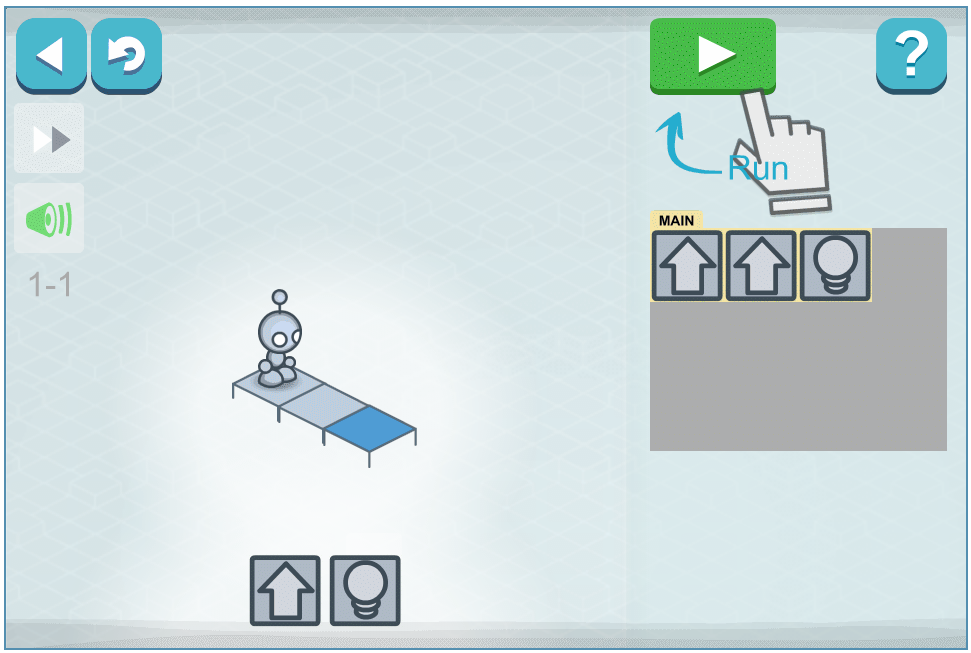
\includegraphics[height=4cm]{img/lightbot-instruction}
\caption{LightBot}
\label{fig:lightbot}
\end{subfigure}%
\begin{subfigure}[t]{0.5\textwidth}
\centering
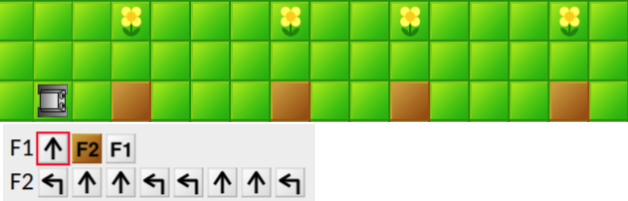
\includegraphics[height=4cm]{img/robotanist}
\caption{Robotanist}
\label{fig:robotanist}
\end{subfigure}
\caption{LightBot and Robotanist provide square grids for commands.}
\label{fig:lightbot-robotanist}
\end{figure}



\subsection{Blockly Games}
\label{sec:blockly-games}
Blockly is a popular block-based programming interface.
In contrast to the blocks in LightBot,
Blockly blocks can be assembled in nested control structures
(\cref{fig:blockly-games}).
Blockly Games%
\footnote{Available at \url{https://blockly-games.appspot.com/}.}
% TODO: Replace by figure using nested control structures
% and move the fre to the end of previous sentence.
%(figure \ref{fig:blockly-instruction})
%demonstrate Blockly usage. The webpage ...
consist of several problem sets with Blockly, ordered by increasing difficulty.
For example, in the first level, students learn how to compose blocks together
as a puzzle, and in the second level they learn loops and conditions by solving
tasks in a maze. Final level serves as a transition from block-based
programming to textual programming in JavaScript.
Each level consists of 5-10 tasks, again ordered by increasing difficulty. %, with no personalization.
The fixed order enables to build on the program from the previous task,
thus gradually leading to more complex programs,
resulting for example in sophisticated images in turtle graphics.
Blockly Games includes non-ignorable interactive instructions,
which require to take a described action before they disappear
\cite{blockly-10-things}.

%\imgW[0.7]{blockly-instruction}%
%  {Blockly Games includes non-ignorable interactive instructions, %
%  which require to take a described action before they disappear.}

\subsection{Hour of Code}
\label{sec:hoc}
Hour of Code%
\footnote{Available at \url{https://hourofcode.com}.}
%(figure \ref{fig:hour-of-code-sw})
provides many one-hour tutorials, each containing about 15 tasks in fixed order,
using Blockly-based language
(\cref{fig:hoc}).
These tutorials focus on motivation, using themes from popular movies and
games, and providing videos with famous people explaining programming concepts.
The tutorials use high-level theme-specific blocks, such as ``set droid to a
random speed``, and they are restricted to only one or two programming
concepts, e.g. sequences of commands and events.
In some tasks, the built program is not a direct solution for a robot,
but rather a game, in which the code specifies actions triggered on events.
% TODO: There is some space to include more info about HoC.

%\imgW[0.7]{hour-of-code-sw}{Hour of Code, Star Wars tutorial.}


\begin{figure}[htb]
\centering
\begin{subfigure}[t]{0.43\textwidth}
\centering
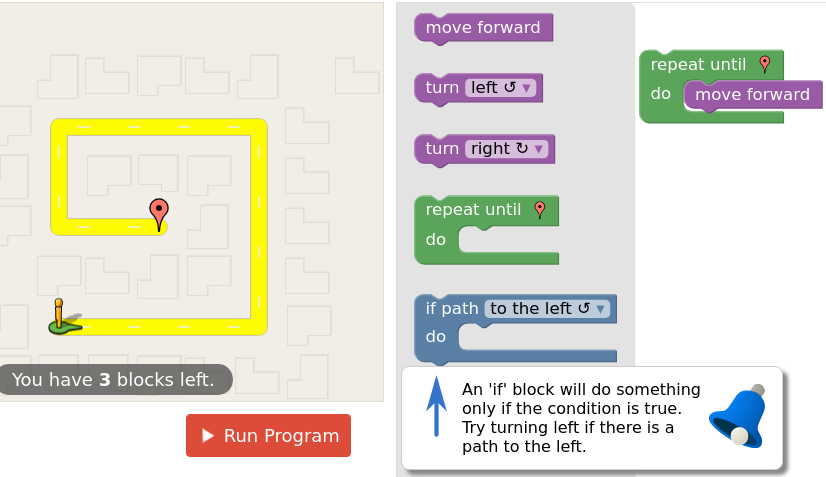
\includegraphics[height=33mm]{img/blockly-nested}
\caption{Blockly Games (Maze level)}
\label{fig:blockly-games}
\end{subfigure}%
~
\begin{subfigure}[t]{0.57\textwidth}
\centering
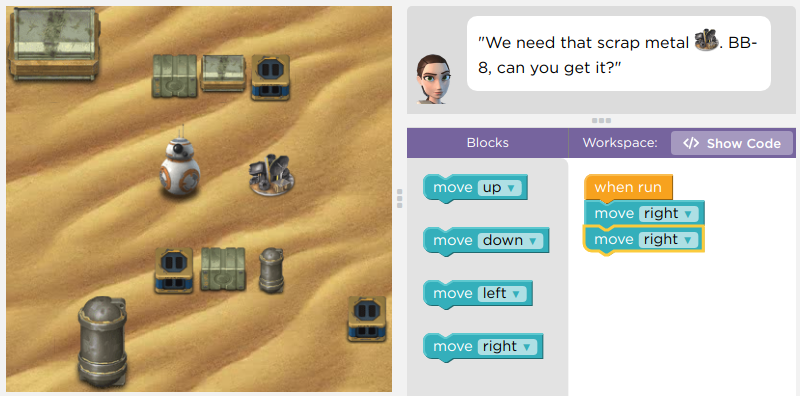
\includegraphics[height=33mm]{img/hour-of-code-sw}
\caption{Hour of Code (Star Wars theme)}
\label{fig:hoc}
\end{subfigure}
\caption{Two programming games using nested blocks.}
\label{fig:blockly-hoc}
\end{figure}





\subsection{Human Resource Machine}
\label{sec:human-resource-machine}
Human Resource Machine%
\footnote{\url{http://tomorrowcorporation.com/human-resource-machine-hour-of-code-edition}}
%\footnote{Free Hour of Code edition available at \url{http://tomorrowcorporation.com/human-resource-machine-hour-of-code-edition}.}
is an example of an offline computer game for learning programming.
%Although it is presented as a game,
%the player spends nearly all the time solving tasks similar to those in the previously mentioned learning systems.
% Removal candidate (1 sentence):
The sequence of tasks is non-personalized and nearly linear,
with a few short side branches.
Similarly to the systems above, it also uses block-based programming,
but now in a different domain:
it offers low-level programming commands, such as
input, output, move-from, move-to, add, or jump
%(figure \ref{fig:human-resource-machine}).
(\cref{fig:hrm}).
% input, output, move-to, move-from, add, sub, jump, jump-nonzero, jump-negative.
The programming environment includes a debugger,
providing a possibility to step through the program.
All concepts are explained when they first appear in the game,
and programming blocks can
be explained again simply by dragging the block onto a dedicated field with a question
mark.

%\imgWithFootnote[0.7]{human-resource-machine}{Human Resource Machine}%
%{Source: \url{https://tomorrowcorporation.com/humanresourcemachine}}
%%{Source: \url{https://tomorrowcorporation.com/humanresourcemachine} (Tommorow Corporation).}

\subsection{Khan Academy}
\label{sec:khan-academy}
Khan Academy has a computer programming curriculum%
\footnote{Available at \url{https://www.khanacademy.org/computing/computer-programming}.}
that uses textual programming in JavaScript with functions for drawing shapes
in absolute coordinates %(figure \ref{fig:khan-academy}).
(\cref{fig:ka}).
In addition to programming tasks, it contains text and video explanations, and
projects. Some videos are in the form of interactive \emph{talk-throughs},
in which the student can fiddle with the explained code at any moment to understand
how it works.

%\imgW[0.8]{khan-academy}%
%  {Parting Clouds programming task on Khan Academy.}


\begin{figure}[htb]
\centering
\begin{subfigure}[t]{0.48\textwidth}
\centering
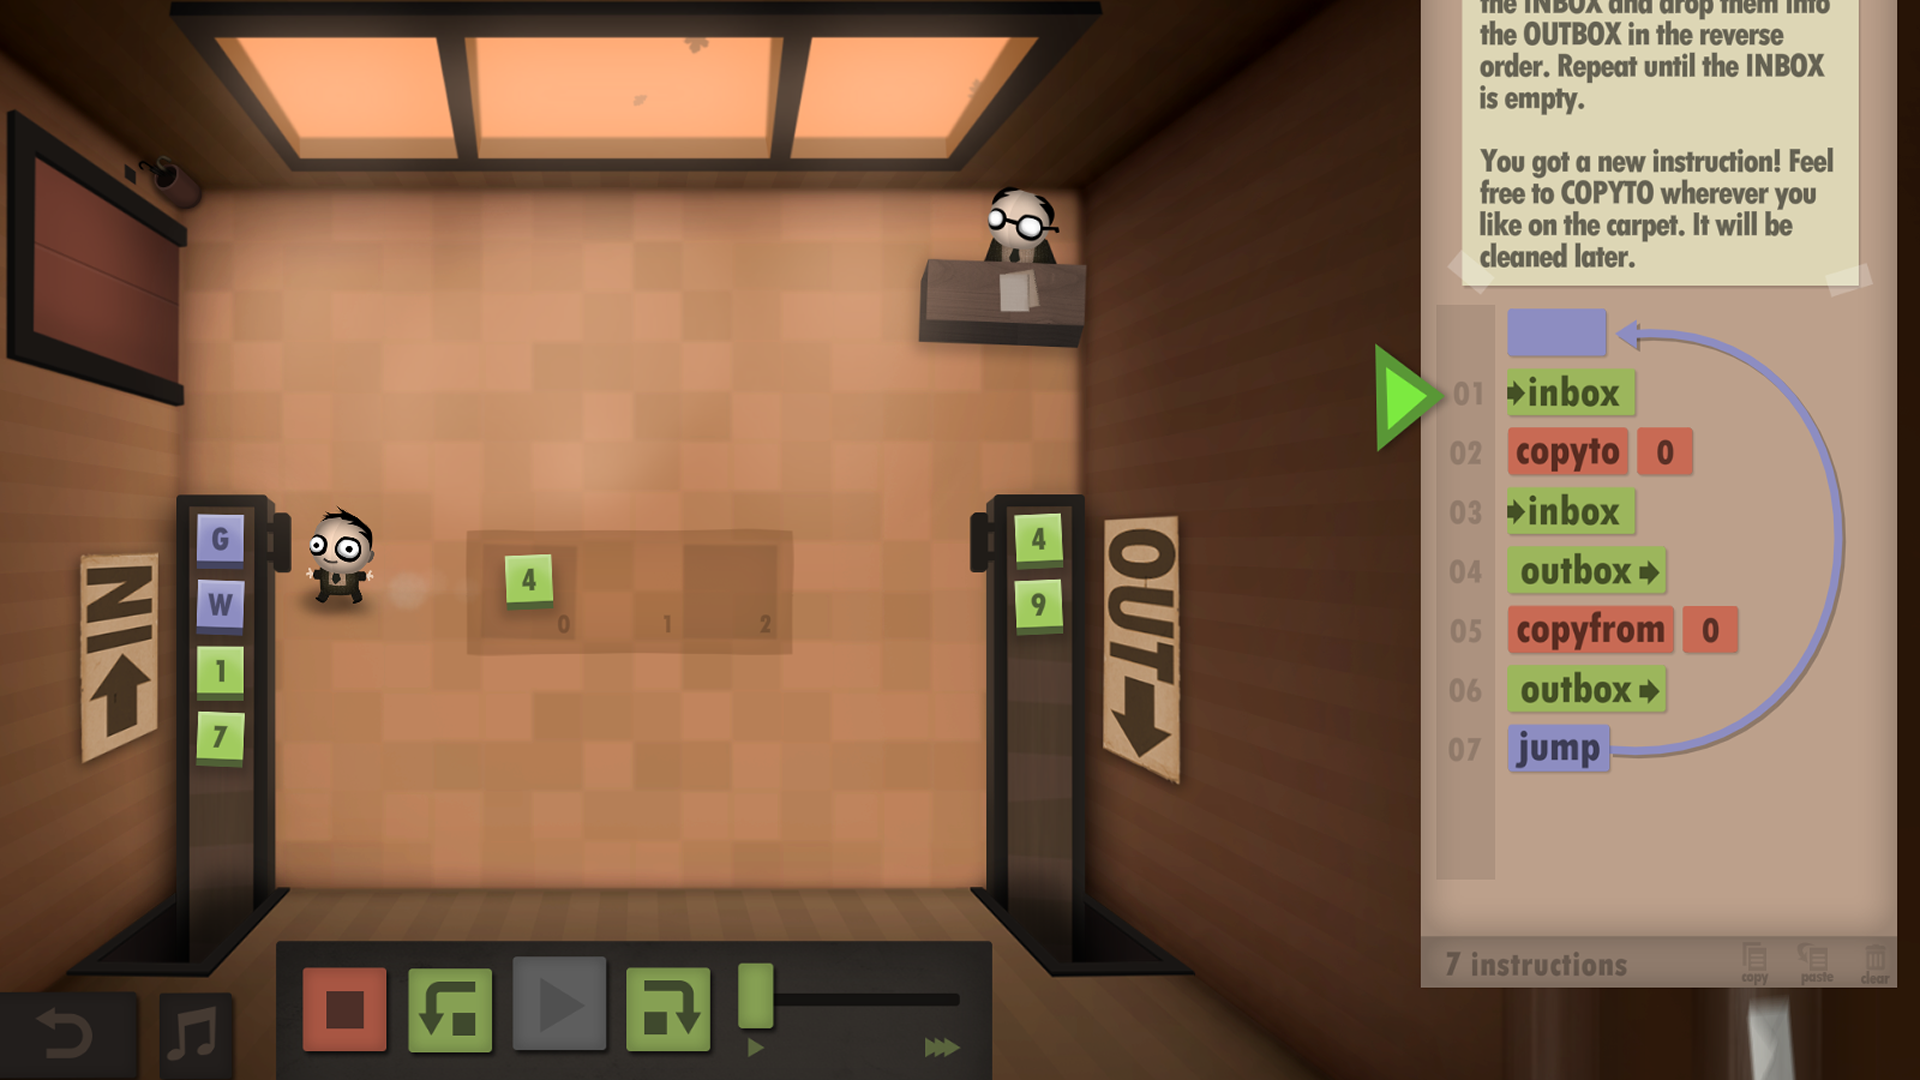
\includegraphics[height=30mm]{img/human-resource-machine}
\caption{Human Resource Machine\protect\footnotemark}
\label{fig:hrm}
\end{subfigure}%
\begin{subfigure}[t]{0.52\textwidth}
\centering
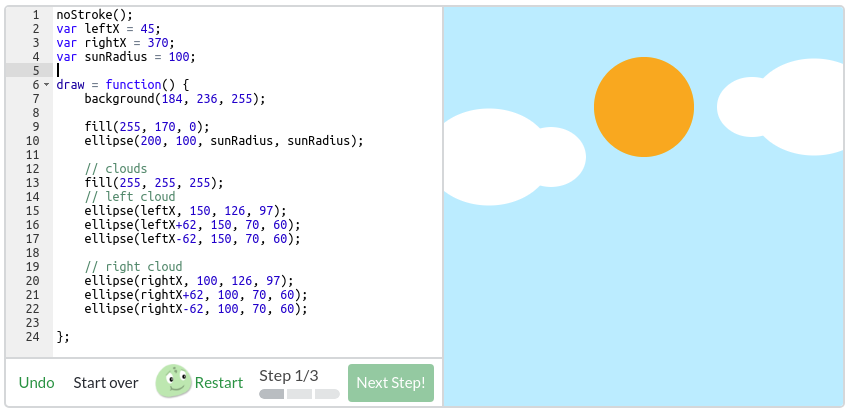
\includegraphics[height=30mm]{img/khan-academy}
\caption{Khan Academy}
\label{fig:ka}
\end{subfigure}
\caption{Tasks using Assembly-based and JavaScript-based languages.}
\label{fig:hrm-ka}
\end{figure}
\footnotetext{Source: \url{https://tomorrowcorporation.com/humanresourcemachine}.}






%\subsection{We Can Code}
%\label{sec:umime}
%
%TODO: present UmimeProgramovat -> turtle graphics, mastery learning
%\footnote{Available at \url{https://www.umimeprogramovat.cz/} (Czech only).}


%\subsection{Ozobot}
%\label{sec:ozobot}
%Ozobot%
%\footnote{Product webpage available at \url{http://ozobot.com/}.}
%is a small physical robot
%programmable by either a Blockly-based interface,
%  or even without a computer
%  by drawing lines on a paper and reading them with a color sensor on the robot.
%As it does not require ability to read and write
%  Ozobot is suitable for even very young children.

%\imgWithFootnote[0.8]{ozobot-robot}{Ozobot}%
%{Source: \url{https://www.flickr.com/photos/robpegoraro/19464353039}, Rob Pegoraro.}

%\imgW{ozobot}{%
%  Ozobot simulator (available at \url{http://games.ozoblockly.com}) %
%  is a Blockly-like interface for creating programs for Ozobot %
%  (but the simulater requires the ability to read). %
%  It also includes a few prepared tasks.}


%\subsection{Project Euler}
%\label{sec:project-euler}
%The core of Project Euler%
%\footnote{Available at \url{projecteuler.net}.}
%is a list of several hundreds of programming problems with one correct answer.
%The problems can be solved in any language
%and then checked whether the computed answer is correct.
%The project is not meant to teach elementary programming,
%but rather to hone one’s programming skills;
%more complicated tasks even require some knowledge of algorithms and data structures.
%
%\imgW[0.7]{project-euler-progress}{%
%Project Euler provides several means of motivation: %
%levels (based purely on number of solved tasks), badges %
%(e.g. for solving 10 consecutive problems, 50 prime numbered problems, etc.), %
%comparison with user’s friends, %
%statistics page with several leaderboard (e.g. by country), %
%and a special score based on the performance on the most recently published problems.}


%\subsection{HackerRank}
%\label{sec:hacker-rank}
%
%Online programming contests,
%in which people attempt to solve as many problems as possible
%in limited time frame of a few hours,
%became popular in the last years.
%In addition to organizing such contests regularly,
%HackerRank%
%\footnote{Available at \url{https://www.hackerrank.com/}.}
%also provides many training programming tasks for various topics,
%from introductory programming to machine learning.
%% Solutions are evaluated on a server against a prepared set of test cases with time limits.
%In addition to the classic motivation in the form of points, badges and leaderboards, students are motivated to practice to perform well in the competitions,
%where they can win some prizes and sometimes even job offers.
%HackerRank also helps student to decide on a problem to solve by showing its difficulty according to the author of the task (on a 3-star scale),
%as well as success rate among the past submissions.
%Furthermore, after solving a task,
%a specific recommendation the next task to solve is shown.


%\imgW[0.6]{hackerrank}{HackerRank. %
%Each task specifies input and output format, including some examples. %
%Solution can be written either locally or in the provided online editor.}


\section{Strategies to Support Learning}
%\section{Strategies for Easier Learning}
\label{sec:strategies-for-easier-learning}

Learning programming is difficult,
  because it requires
  to adopt algorithmic thinking,
  understand program execution,
  and remember formal syntax of a programming language;
  all these three skills at once. % at the same time.
To make learning easier,
  the systems presented in the previous section use diverse strategies,
  such as avoiding syntax errors,
  displaying visual output
  and providing hints.
Various other strategies were tried in the past as well;
article \emph{Lowering barriers for Novice Programmers}
  \cite{lowering-barriers}
  provides a detailed overview.


\subsection{Avoiding Syntax Errors}
\label{sec:avoiding-syntax-errors}

A common strategy for avoiding syntax errors is to replace textual programming
with drag-and-drop block-based programming.
There are two basic types of block-based interfaces:
  either with a square grid defining the program shape,
  often one row per function
  (\cref{fig:lightbot-robotanist}),
  or the blocks can be nested and assembled arbitrarily,
  with no limit on maximum program length,
  often one vertical stack per function
  (\cref{fig:blockly-hoc}).
The fixed square grid is simpler to understand and manipulate with,
  but it does not allow for nesting,
  which is a fundamental feature of computer programs.
This restriction is usually overcome by
  combining condition and commands into a single block,
  by using recursion instead of loops,
  and by replacing nested sequences of commands by a new function.

%TODO: the block-based editors are a special case of "structred editors",
%idea: editor only allows edits that transform the code from one syntactically correct
%program to another (basically working on AST level, edit = transforms to another AST)
%(compared to: classical text editors, where the edit can be arbitraty, making the code
%not syntactically correct).

%\subsection{Potential Drawback of Block-based Interfaces}
%\label{sec:potential-drawback-of-block-based-interfaces}
A drawback of using block-based programming
  is that the students need to learn a proper textual programming language in
  the future to be able to implement more complex programs.
Several controlled experiments were performed to test a hypothesis
  that it is still beneficial to start an introductory programming course
  with a block-based programming,
  even when the students will be writing textual code later in the course
  \cite{comparing-blocks-text-price2015, comparing-blocks-text-weintrop2017}.
Results suggest that block-base interfaces indeed lead to increased learning and
motivation; however, the evidence is not fully convincing. For example, in
some of these studies, the programming interfaces differed in more aspects than
just in using blocks instead of text. Furthermore, these studies do not
answer when it is the right moment to switch from block-based to textual
programming.

%\subsection{Transition Strategy}
%\label{sec:transition-strategy}
%Weintrop and Wilensky suggest that the block representation of the code
To make the transition easier, block representation of the code
  should match the underlying programming language
  to which the student is expected to move in the next phase
  \cite{challenges-of-blocks-based-environments}.
However, resemblance to a programming language sometimes
  conflicts with the readability of the blocks for novices.
Instead of making compromises,
  the system can progressively change the available set of blocks in each level,
  making them more and more similar to a textual programming language.
In the last level of Blockly Games, which employ this strategy,
  the text on the blocks matches the generated JavaScript exactly
  \cite{blockly-10-things}.

%TODO:
%- note: "blending block-based and text-based programming approaches (e.g., Pencil Code
%(Bau 2015), Tiled Grace (Homer and Noble 2014), and Greenfoot’s Frame-based editor (Kölling et al.
%2015)"


\subsection{Visual Output}
\label{sec:visual-output}

Learning systems can help students to track program execution
  by providing a clear visual representation of the current state
  and effects performed by the program.
This can be achieved naturally for turtle graphics,
  where the whole state is just a position and orientation of the turtle,
  and effects are the drawn lines.
Similarly, in simple games, such as those described in
  \cref{sec:lightbot,sec:problem-solving-tutor,sec:blockly-games,sec:hoc},
  the grid world visualization contains complete information about the current
  state (\cref{fig:lightbot-robotanist,fig:blockly-hoc}).
For the simplicity of their visual output,
  drawings and grid world games have become prevalent task types
  in the current systems for learning programming.

\subsection{Instructions and Hints}
\label{sec:instructions-and-hints}

Most educational systems include instructions
  to explain new concepts such as loops and conditions.
%However, Neil Fraser explains that students ignore instructions,
However, many students ignore instructions,
  no matter how prominent they are \cite{blockly-10-things}.
A solution to this problem are actionable non-ignorable instructions,
  which cannot be closed manually by the student, and disappear only once the
  student performs the action described in the instruction
  (\cref{fig:blockly-games}).

In addition to the instructions, some systems offer hints, which appear either
  upon a student request, or automatically after a certain time of unsuccessful
  solving. Although it is possible to generate a hint in any state,
  using data of students which have successfully solved the task before
  \cite{generating-hints}, the existing systems use a few manually prepared
  hints, instead of relying on the automatic approaches.

\section{Strategies to Support Motivation}
%\section{Strategies for Motivation}
\label{sec:motivation}
% NOTE: Prev section: learning, this section: engagement.

In addition to strategies for easier learning presented in section
\ref{sec:strategies-for-easier-learning}, it is equally important to create an
engaging environment supporting students’ motivation.
All strategies for supporting motivation are based on fulfilling some human
needs \cite{nvc}. % TODO: cite specific page
\Cref{tbl:motivation-strategies} links needs to common strategies.
% TODO? related: flow, happiness, switch-elephant (prev. section: path)

\begin{table}[htb]
\centering
\begin{tabular}{ll}
\toprule
Needs & Strategies \\
\midrule
Purpose & Emphasizing usefulness of the programming skill. \\ %, confidence
Progress, learning & Skills visualization, points, levels. \\
Effectiveness & Recommending tasks of optimal difficulty. \\ % concentration/flow
Autonomy & Allowing to choose a topic or a task. \\
Recognition & Badges, leaderboards. \\  %Appreciation  % leaderboard vs. scoreboard?
Sharing & Possibility to share programs or achievements. \\
Cooperation & Pair programming. \\
Beauty, harmony & Appealing game world. \\ %, which is nice to look at and fun to play with \\
Fun & Entertaining tasks. \\
Creativity & Open-ended tasks, projects. \\  %, self-expression
% Community?
\bottomrule
\end{tabular}
\caption{Needs and strategies that help to fulfill these needs.}
\label{tbl:motivation-strategies}
\end{table}



\subsection{Appealing Game World}
\label{sec:motivation.game-world}
Ideally, game world should appeal to students --
even without tasks to solve,
  it should be an interesting toy to play with \cite{book-of-lenses}.
That is why all Hour of Code tutorials are based on movies and games
  popular among children, such as Angry Birds, Frozen, or Star Wars
  (\cref{fig:hoc}).
In such environments, it is possible to assign open-ended tasks,
  or even let the students create whatever they want,
  which works well especially for creative students seeking for self-expression.
For example, Khan Academy programming curriculum contains many several
open-ended drawing projects (\cref{fig:ka}).
%\cref{sec:robomission.game-world}

\subsection{Entertaining Tasks}
\label{sec:motivation.tasks}
For many students, giving them specific small problems works better
  than large, loosely defined, open-ended tasks.
By solving small problems quickly,
  they get a feeling of progress and learning.
Another advantage of closed tasks
  is a more straightforward implementation of gamification features and adaptive behavior.

Small closed tasks result in short programs,
  but their behavior should be still interesting. % for the students to be satisfied.
To achieve complex behavior,
  a system can either provide students with macro-commands (e.g. to draw a circle)
  or with a skeleton of complex code, with a few gaps to fill in by students.
However, it is important for the students to feel ownership over the code,
  which is especially a concern with the code skeleton.
Solution implemented in Blockly Games
  is to make a series of tasks in which the students
  build on their program from the previous task
  \cite{blockly-10-things}.

% TODO: some examples in the form of figures + descriptions
% TODO: other important aspects: variability


\subsection{Optimal Challenge}  % OR: "Optimal Difficulty"
\label{sec:motivation.challenge}
For a great learning experience,
  difficulty of the task must match the skill of the student.
If the task it too easy,
  the student is not challenged and gets bored.
If the task is too difficult,
  the student becomes frustrated and desperate.
On the other hand, if the task has appropriate difficulty,
  the student is likely to be challenged and focused
  (\cref{fig:flow}).
The complete immersion into the task the student is solving at the moment is called
  a state of flow \cite{flow},
  or a \emph{zone of proximal development} \cite{zone-of-proximal-development}.
Achieving the state of flow maximizes the learning outcome \cite{adaptive-practice}.
  % and even increases the long-term level of happiness. % TODO: find a source of this claim
\Cref{chap:adaptive-learning} describes techniques for estimating student's skills
and recommending tasks of optimal difficulty.
% for estimating student’s skill and show how to use that estimate for task recommendation and mastery learning.


\subsection{Gamification and Progress Visualization}

Sense of progress and learning can be boosted by visualizations of
progress towards mastery in the current topic, solved tasks, completed problems sets,
or acquired skills.
\Cref{fig:progress-visualization} shows examples of progress bars from various systems.

% TODO: cite relevant research, open learner model
% NOTE: also helps to decide what to practice next, while preserving student's
% autonomy (soft recommendation)

\begin{figure}[htb]
\centering
\begin{subfigure}{.48 \textwidth}
  \centering
  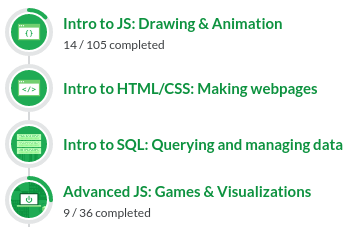
\includegraphics[width=.9\textwidth]{img/ka-skills}
\end{subfigure}
\begin{subfigure}{.48\textwidth}
  \centering
  
\includegraphics[width=.9\textwidth]{img/hour-of-code-progress}
  \bigskip
  \vspace{1mm}
  
\includegraphics[width=.9\textwidth]{img/umime-progressbar}
\end{subfigure}
\caption{%
  Progress bars: Khan Academy topics, Hour of Code tutorial,
  and mastery progress bar in Umíme Programovat (``We Can Code'').}
\label{fig:progress-visualization}
\end{figure}


%\subsection{Gamification}

Although the programming tasks themselves can be considered as a game
(e.g. Human Resource Machine from \cref{sec:human-resource-machine} is
presented purely as a game),
most learning systems add further gamification elements to increase the sense
of progress.
Common gamification elements include points, levels, badges, and leaderboards.

% TODO: figures: Project Euler, KA
% TODO: ref relevant research

\chapter{Adaptive Learning}
\label{chap:adaptive-learning}

% TODO:
% - incorporate other notes from my/thesis gdoc
% - inspiration from relevant articles
% - add references for provided examples (playing chess, autonomous car, ...)

Artificial intelligence proved to be a mighty tool
  for tackling difficult algorithmic tasks,
  from playing chess to driving an autonomous car.
The power of artificial intelligence can be also used
  to develop a personalized adaptive system for learning programming.
Such system should create an optimal learning experience for each student
  by providing them with problems of difficulty matching their skill,
  so that the student stays challenged and interested in solving them.

In the existing systems (\ref{sec:existing-systems}),
  the sequence of tasks is the same for everybody.
As a result, the progress is necessarily too slow for some students,
  who could skip some of the tasks,
  while being too fast for others,
  who could highly benefit from solving many more similar tasks.
Artificial intelligence can be used to personalize
  the sequence of tasks for every student.
By giving the student a suitable task
  -- neither too easy, nor too difficult --
  it can help the student to get into the state of flow
  (\ref{sec:motivation.challenge}).

In addition to choosing the most suitable task for given student,
  artificial intelligence has also other possible uses in learning systems,
  for example automatic hints generation \cite{generating-hints}
  or skills visualization (TBA: ref).
Furthermore, artificial intelligence techniques can be used
  to analyze collected data offline
  and, for example, detect problematic tasks
  or suggest how to group tasks into categories (TBA: ref).

Adaptive learning systems have been already successful in some domains.
For instance, Map Outlines%
  \footnote{Available at \url{https://outlinemaps.org}.},
  developed by Adaptive Learning research group at Masaryk University,
  is an intelligent web application for learning geography.
It has been used by tens of thousands of students
  and online experiments have confirmed
  that the adaptivity of the system helps to improve the learning outcome
  \cite{alg.evaluation-geography}.
In addition to geography, similar adaptive web applications
  for learning anatomy%
  \footnote{Available at \url{https://practiceanatomy.com}.},
  biology%
  \footnote{Available at \url{https://poznavackaprirody.cz} (in Czech only).},
  elementary mathematics%
  \footnote{Available at \url{https://matmat.cz} (in Czech only).},
  and Czech grammar%
  \footnote{Available at \url{https://umimecesky.cz} (in Czech only).},
  were developed by the research group in recent years.

Section \ref{sec:student-modeling} presents how to model students
  in the context of learning programming.
Sections \ref{sec:task-recommendation} and \ref{sec:mastery-learning}
  then describe how to use these models to make a learning system adaptive.
Finally, section \ref{sec:metrics-and-evaluation} discusses how to evaluate
  different models or even whole learning systems.


\section{Student Modeling}
\label{sec:student-modeling}

For the system to be adaptive, models of
  a student skill, task difficulty, and student-task interaction
  need to be designed, implemented and evaluated using collected data.
The purpose of these models is to predict the probability that a given student
  would solve a given task
  and also the time the student would need to complete the task.


\subsection{Data}
\label{sec:student-modeling.data}

To learn model parameters, such as difficulty of individual tasks, some data is needed.
What data is needed and how much differs across models.
Some data about tasks are independent of students;
therefore, they can be obtained in advance,
which can be useful for initial task difficulties estimates.
Three types of task data are distinguished:

\begin{itemize}
  \item task statement (including name and world description),
  \item sample solution (or multiple solutions),
  \item expert labels (e.g. covered concepts).
\end{itemize}

Task statements are always available,
  because they are needed to present tasks to students.
However, obtaining sample solutions and expert labels
  incurs additional costs for a new system.
% TODO: Note that quite often, systems needs sample solutions and some labels
%       for the presentation purposes anyway.
Moreover, they can be noisy and imperfect.
For example, an annotator can forget to include some labels
  or even make a mistake in the sample solution.

Once the task is deployed in the running system,
  rich data can be collected from each interaction between a student and a task:
\begin{itemize}
  \item whether the task was eventually solved,
  \item solving time,
  \item number of clicks, number of code executions,
  \item program snapshots (e.g. after each code change),
  \item rating or labels provided by the student (e.g. perceived difficulty).
\end{itemize}

% TODO: also consider to include hints in the list
% TODO: mention different granularity levels for taking program snapshots (+cite)

\subsection{Item Response Theory}
\label{sec:irt}

The simplest version of item \emph{item response theory} (IRT)
  \cite{irt-visual-guide}
  models each student by a one-dimension skill $s$,
  and each task by a one-dimension difficulty $d$.
IRT assumes that the probability of a student with skill $s$
  successfully solving a task with difficulty $d$
  is given by the following function:
  \begin{equation}\label{eq:logistic}
  P(s, d) = \frac{1}{1 + e^{-(s - d)}}
  \end{equation}

% TODO: mention 2-parameter model (explain discrimination parameter)
\begin{figure}[h]
  \centering
  \begin{tikzpicture}[domain=-2:4, smooth, samples=20, scale=1]
  \draw [thick, ->] (-2,0) -- (4,0) node [below right] {$s$};
  \draw [thick, ->] (0,0) -- (0,2.5) node [left] {$P(s,d)$};
  \draw [thick] (-0.1,1) node [left] {$0.5$} -- (0.1,1);
  \draw [thick] (-0.1,2) node [left] {$1$} -- (0.1,2);
  \draw [thin, dashed] (0,2) -- (4,2);
  \draw [thin, dashed] (0,1) -- (1,1) -- (1, 0);
  \draw [thin, dashed] (-0.57,2) -- (-2,2);
  \draw [thick] (1,0.1) -- (1,-0.1) node [below] {$d$};
  \draw [very thick] plot (\x, {2 / (1 + exp(1 - \x))});
  \end{tikzpicture}
  \caption{One-parameter Unidimensional Logistic Model}
  \label{fig:logistic-model}
\end{figure}

This basic model was originally developed for a simple knowledge testing
  and therefore it assumes a single constant skill.
However, programming skill is multidimensional;
  for example, one student can be proficient with functions and struggle with loops,
  while another student can master loops and struggle with functions.
Furthermore, these skills should be ideally changing significantly during
  the interaction with the system, because students are learning.

Another drawback of the IRT is that it only uses
  the binary data about successes and failures.
As nearly all interactions in programming learning systems end with a solved task,
  it would be more useful to work with solving times,
  which can provide more information about students' skills.

Item response theory can be extended to overcome these limitations.
\emph{Problem Response Theory} (PRT)
\cite{alg.problem-response-theory, pelanek-student-modeling-times}
% TODO: only cite the more relevant paper (or extend this section and cite both
% on relevant places)
predicts problem solving times instead of probability of success,
assuming an exponential relationship between a problem solving skill
and the time to solve a problem.
PRT can be formulated to use multidimensional skills.
The model parameters (skills and difficulties) can can be estimated from the data
  using one of the \emph{maximum likelihood estimation} algorithms.
  % TODO: cite paper describing the parameters estimation (or MLE?)
% (for IRT, it's \cite{irt-theory-and-practice}, but PRT would be better)

% TODO: find and provide the details about the learning extension of PRT
% (isn't it already the elo?)

% TODO: Add note that the assumption of exponential relationship is justified
% by observed solving solving times distribution and it is also intuitively
  % plausible - multiplicative nature of solving times.



\subsection{Elo}
\label{sec:elo}

The Elo model \cite{alg.elo}
  extends the logistic model presented in section \ref{sec:irt}
  to capture changing knowledge.
The model is inspired by the rating of chess players \cite{elo-rating}.
It interprets each attempt  to solve a task
  as a ``match'' between the student and the task
  and after this match ends, skill and difficulty estimates are revised.

If the student solves the task faster than expected by the model,
  their skill is increased and the difficulty of the task is decreased.
On the contrary, if the student fails to solve the task or if takes them too long,
  their skill is decreased and the difficulty of the task is increased.

% TODO: formulas (for time-variant of elo)
% TODO: mention differnet updates for tasks (exponentially decayed) and
% students (their skill is assumed to change and not converge)

The main advantage of using the Elo model is its simplicity, flexibility,
  good performance and intrinsic online nature, which allows for immediate
  updates of parameters as students are interacting with the system.

% TODO: include other models, PFA, BKT etc.


\subsection{Concepts}

% TODO: consider to move this section before the description of individual
% models
% TODO: fix and mention used terminology: concept vs. skill

A lot of research in the field of adaptive learning
  restricts its attention to a one-dimensional skill.
This assumption is reasonable for many logic puzzles (e.g. sudoku);
however, solving programming tasks requires diverse skills.
Even in the introductory programming, loops, conditional commands and functions
  can be taught in any order
  and it is perfectly possibly to master one of these skills,
  while struggle with the others, or even not been introduced to them.

As we mentioned in sections \ref{sec:irt} and \ref{sec:elo},
  both the IRT and Elo models can be extended to work with multidimensional skills.
% TODO: However, the way they compose multiple skills into a single prediction
% is not completely justified / can differ depending on domain/skills (e.g.
% adding skills vs taking best/worse)
Although modeling multiple skills seems useful,
  there is a trade-off between the complexity of the model (number of skills)
  and how well (or how fast) can be the parameters estimated.
More parameters require more data and time for the estimates to converge.
% TODO: which is especially concern for students; 1. predictions needed
% immediately for new students (no/little data), 2. students' skills are
% assumed to change (tasks didn't have these problems)


% \subsection{Learning Concepts from Data}

Concepts can be either defined manually or detected automatically
  \cite{niznan-thesis}.  % TODO: specify chapter/pages
Manually selected concepts, such as loops and conditional commands,
  have the advantage of being interpretable,
  so they can be used for skills visualizations in the user interface
  to provide students with the information about their learning progress.
Furthermore, no data needs to be collected in advance,
  while the automatic techniques require a lot of data to provide stable results.  % TODO: how much?


% \subsection{Prerequisites}
Undoubtedly, there are some relationships between skills;
  for example, nested loops cannot be mastered without mastering simple loops.
The hierarchical structure between concepts can be modeled
  as a directed acyclic graph (DAG),
  where each vertex is a concept and each edge represents a prerequisite.
Having DAG of concepts then allows to model students using Bayes networks
  \cite{its-programming}.

% TODO: simple diagram: DAG of concepts example

\section{Task Recommendation}
\label{sec:task-recommendation}

Student models are used by an \emph{instructional policy} to recommend
  the most suitable task for a student.
In spite of having all the predictions about success probabilities
  and time estimates in hand,
  task recommendation is not an easy task.
First, it is not clear what the optimal difficulty even means.
Second, it may vary for different students, domains or types of problems.
Furthermore, optimal difficulty is not the only criterion to be considered.
For instance, diversity of tasks is important to keep students interested.
No principled techniques for task recommendation have been developed yet;
however, several heuristic approaches have been used
  and proved to work well (TBA: ref).

Task recommendation is not a necessary requirement
  for the system to be adaptive.
Student models can be utilized by other means to achieve personalized behavior,
  e.g. in mastery learning (section \ref{sec:mastery-learning}).
The system can also just provide students with predicted solving times
  and let them to choose the next task they want to tackle.

Showing predictions can be already perceived as a very mild form of recommendation.
Indeed, recommendations can range from \emph{soft} to \emph{hard}.
Soft recommendations can be achieved either by
  ordering tasks according to suitability,
  filtering and only showing a subset of tasks,
  or showing suggestion such as
  ``too easy'', ``too difficult'' and ''ready to tackle'' next to each task.
For example, suggestions in the form of traffic-light colors
  are used in the system described in \cite{its-programming}.
The system can be more strict and show only a single recommended task,
  or even enforce the recommendation by immediately progressing student to
  the next task without asking and giving them a chance to select a different task.

\bigskip
\emph{TODO:\\details about techniques (heuristics, methods) for selecting single best task}

\section{Mastery Learning}
\label{sec:mastery-learning}

\emph{TODO:\\describe mastery learning + usage of student models%
(to show the progress and to determine that the student already achieved the mastery)}

% TODO: screenshot of a mastery progress bar (e.g. from UmimeX)

\section{Metrics and Evaluation}
\label{sec:metrics-and-evaluation}

To decide if the adaptivity of the system increases the learning outcomes,
  a suitable metric must be chosen and incorporated into the system,
  for example using pre-tests and post-tests.
Ideally, the system should also allow to easily change various conditions
  for subsets of students and hence perform controlled online AB experiments.


\subsection{Metrics for Predictions}

\emph{TODO}

%TODO: data we need -- this is simple: we can collect the objective solving times and compare
%with predictions (there is some noise, because of students taking breaks, cheating, etc., but should be ok)
%
%TODO: mention standard metrics and evaluation methodologies in ML (for
%predicted times, RMSE vs. MAE etc.)


\subsection{Metrics for Recommendation}

\emph{TODO}

%TODO: what data to use? much less clear than  for predictions
%
%TODO: mention standard metrics and evaluation methodologies in RC (for recommended tasks)
%
%The tasks environment in learning systems often differ significantly
%  from the real-world environment,
%  e.g by using blocks instead of text
%  and other aspects mentioned in section \ref{sec:strategies-for-easier-learning}.
%This makes evaluation harder, because while the collected data on which we
%  evaluate the system comes from the system itself,
%  ultimately students leave this simplified environment
%  and the performance outside the learning system is the important criterion.

% This issue is mentioned in \cite{challenges-of-blocks-based-environments},
% by Werntrop and Wilensky
% in the context of proper evaluation of block-base programming environments.

% TODO: this relates to next subsection on ultimate goal vs. proxy metrics
% TODO: also consider short discussion on high-level vs. low-level goals
% (also known as mission/purpose/vision vs goals, or goals vs means
% and discussion on goals vs metrics



\subsection{Ultimate and Proxy Metrics}

\emph{TODO}

%TODO: explain possible metrics derivation: -- with specific example of learning programming
%1. from the ultimate goal (vision, mission) -- but make it precise to make it evaluable (if had all the data we need)
%2. proxing 1 to make it measurable in the long term (AB experiment)
%3. proxing 2 to make it measurable in the short term (live evaluation)
%4. proxing 3 to make it work with offline data (to learn hyperparameters + for holdout evaluation)
%5. proxing 4 to make it differentiable function (to guide learning, ie. for updates after new s-t interaction)



\subsection{Perceived Flow}

\emph{TODO}

%Instead of using objective (factual, measured) data (such as solving time),
%we can ask students to provide explicit ``rating'' (subjective/perceived difficulty),
%  e.g. by selecting tags after solving a task,
%  such as ``too easy'', ``too difficult'', `just right''
%  (or possibly even more specific such as ``boring'', ``weird'', ``fun'').
%Advantage: flow looks as a good proxy metric to optimize.
%Disadvantages:
%  bother students with another questions,
%  takes time (but this is negligible comparing to solving programming task),
%  inaccurate (noise depending on the mood etc.)
%


\subsection{Iterative Improvement}
\label{sec:iterative-improvement}

\emph{TODO}


%TODO: explain importance of offline analysis and monitoring;
%TODO: the term ``human in the loop'' \cite{stupid-tutoring-systems-intelligent-humans}
%TODO: AB experiments
%TODO: importance of iterative improvement, rule of the loop;
%TODO: provide more details -> extend to a section

\chapter{Design of Programming Game}
\label{chap:design-of-game}

%% Terminology + importance.
Design of a programming game deserves a careful attention,
because tasks are the most important part of a system for learning programming.
%...since...
They are the means for learning,
and students spent nearly all the time in the system by solving them.
% TODO: terminology: game, task, PS
% NOTE: rule of the loop + strategy: prototyping several ideas, measure
% metrics to see which games work best.

%% Requirements.
% ... "Therefore" (to link it to the importance in prev paragraph)
To support engagement, tasks must be fun, entertaining,
and immediately appeal to be solved.  % TODO: Fix English.
%(TODO: mention how we underestimated the importance of the entertaining tasks in the first prototype)
To enable learning, the game must allow for tasks requiring all basic
programming concepts, such as sequence of commands, loops, and conditional
statements. % repeat, while, if, if-else, simple tests (comparing)
To enable outer-loop adaptive behavior, multiple diverse tasks practicing same
concepts are needed, including a lot of tasks using only sequences of commands
without more advanced programming constructs.
% (TODO?: other requirements mentioned in the prev. chapters (+REF?)

% TODO: Ideally, mimic and refer to the sections in the chapter on Learning Programming
% (how we incorporated the strategies for easier learning and for motivation)

We have designed a simple game which is a variation on a robot
on grid with a space theme, and which uses Blockly for building programs
(\cref{fig:robomission-task2}).
This choices support all main strategies for easier learning of programming
(\cref{sec:strategies-for-easier-learning}),
including
avoiding syntax errors by using block-based programming,
showing a visual output (the grid world),
and providing short instructions and explanations. % TODO: elaborate?
We combine several strategies to support motivation (\cref{sec:motivation}),
such as appealing game world, entertaing tasks, progress through levels,
and recommending tasks of optimal difficulty
(adaptivity is discussed in \cref{chap:design-of-adaptivity}).
% TODO: target group: Currently, the system primarily targets at children
%  between 10-15 years? (or simply primary school)

% TODO: Img: English localization.
\imgW[0.9]{robomission-task2}{RoboMission, Zig-zag task.}

% NOTE: rule of the loop \cite{book-of-lenses}

\section{Game World}  % Space World
\label{sec:robomission.game-world}

The game world itself should be pleasure to look at and fun to play with,
even without a specific task to solve \cite{book-of-lenses}.
We have based the game world on a popular choice of a robot on grid,
using a theme of a spaceship flying through space and collecting diamonds
(\cref{fig:spaceworld}).
% TODO: better word than "popular"?
%% Game elements.
Each field in the \epmh{space world} has a background color, which
the spaceship can read and use for decisions (e.g. turning left on red fields).
In addition to the spaceship controlled by the student,
there are a few other game objects, that can reside on one of the fields.
These are diamonds, that need to be collected,
large asteroids, that cause spaceship to crash if it hits them,
small meteoroids, that can be shooted,
and wormholes that serves as teleports.

The spaceships start on the bottom row and it always moves one row forward
after any action. % towards its final destination (the last row).
% TODO: elaborate / illustrative figure showing a step and a path
In addition to flying and turning, the spacehsip can also shoot small meteroids.
Having these four basic actions (fly, left, right, shoot) already allows for a
diversity of simple tasks which only practice sequence of commands.
% TODO: limited energy, in order to force thinking about whether to fly or shoot
The spaceship has two sensors, one for the color under the spaceship, and
second for its horizontal position (column index). Having two different sensors allows
for diverse tasks practicing conditions, including testing inequalities, and
potentially also compound conditions.

An inovative feature of the game is the default forward movement,
%where turning results in a shift to a neighboring column
%and each action (including turning) are linked with a forward movement.
which results in shorter programs.
For example, to fly around a stone, only two commands are needed % (left, right),
instead of either 4 or 8 (depending on whether the available commands include
movement in any of the four directions, or only forward movement and turning)
(REF:fig).
% 4: LFFR (e.g. in StarWars game), 8: LFRFFRFL
% TODO: or 4 as a semi-step (single direction OR default movement)
Furthermore, as the spaceship is always facing up, a common left-right
confusion is mitigated (CITE).

%\item movement -- always 1 row forward ("continuous flight ahead") --
%  advantages:
%  (1) mitigates ubiquitous left-right turning confusion;
%  (2) shorter programs (REF example);
%  disadvantages:
%  (1) this behavior is different than what most users initially expect
%  (2) underutilization of fields (only 1 field in each row and only once)
%      (leading to long worlds).
%\item chosen remedy for the 2nd disadvantage: worm holes
%  % (another possibilities: multiple spaceships, long worlds)

%\begin{itemize}
%\item original version - robot-in-maze, issues:
%  \begin{itemize}
%  \item not flexible and did not allow for a lot of diverse easy tasks,
%  \item which is crucial for adaptive learning system
%  \item unnecessarily long programs for simple ideas (non-elegant programs) (TBA: show comparision)
%  \item non-elegant tasks
%  \item ugly worlds
%  \item not very original and entertaining for kids
%  \end{itemize}
%\item requirements (on the topic/theme/world):
%  \begin{itemize}
%  \item entertaining for children
%  \item allowing to create plenty of diverse (and entertaining) tasks, inluding very simple ones
%  \item programs should be not too verbose
%  \item not limiting adaptability (e.g. story requring a fixed sequence of tasks would be a problem)
%  \item (not limiting another topics later)
%  \end{itemize}
%\item fully observable world
%\item no chance (randomness would complicate evaluation and interpretation
%  of data) (there is still some \emph{surprise} in the game for the players:
%  ``Will my program solve the task or not?'')
%%\item REF to formal grammar for the space world in the next chapter
%\end{itemize}

% TODO: use different spaceworld than in Imlementation chapter.
\imgW[0.28]{spaceworld}{Examples of Space World. TODO: add more spaceworlds}


%\imgW{prototype-pits}{Lesson from the first prototype: world must contain
%elements that the program cannot check to enable diverse tasks. As we had a
%natural sensor to check walls, we needed to add pits that could not be checked
%by any sensor.}


\section{Tasks and Programs}
\label{sec:robomission.programs}

intuitive and clear goal: reach last row (blue line), collect all dimanods

\begin{itemize}
\item Given an instace of a spaceworld as described in the previous section
(input), the goal is to create a program for the spaceship such that it reaches
the final row and collects all diamonds on the way.
\item Form of the program: Blockly blocks (+ potentially RoboCode based on
Python, ref to grammar in next chapter; ref to Blockly in prev. chapters)
\item Available blocks: depends on the level;
  actions (...), sensing (...), repeat, while, if, if-else.
\item execute current program any time until correct
\item limits: ``lines'', energy.
  (TODO: explain what they are and why/when they are needed).
\item Why line-limit instead of block-limit: too many blocks (consider while
  loop with a compound condition), so it becomes even difficult to count;
  while the number of lines is always reasonable.
  Bonus: the limit can be directly used for text-based programming as well.
\item TODO: design decision: similar to Python as much as possible: for easy transition
(see the transitional strategies section in chapter 2), allows for AB experiments
comparing directly the influence of the text/block environment as done e.g.
in the field study in \cite{comparing-blocks-text-weintrop2017}.
\end{itemize}


\section{Instructions and Explanations}

\imgW{robomission-mini-instruction}{When a student encounters a new programming concept or programming element, the system displays a short instruction.}
\imgW{robomission-mini-explanation}{The system shows an explanation why the exection was unsuccessful.}
\imgW{prototype-instructions}{Instructions in the first prototype. Nobody was reading them. Most people even did not notice there are any instructions.}


\section{Game Editor}  % OR: task editor?
\label{sec:robomission.task-editor}

A part of the system is at task editor (REF: image)
that enables to easily create new tasks.
(TODO: mention how inconvenient it was in the first prototype, especially the tokens...)
(TODO: mention that the task editor is part of the public site, so anybody can create a task, provide a link and ref to details about task format in the next chapter)


\imgW{task-editor}{Task editor allows to create new tasks.}
\imgW{task-editor-vim}{Task editor allows to to write solutions in Python-based RoboCode and edit space world in Vim mode.}

\chapter{Design of Adaptivity}
\label{chap:design-of-adaptivity}

\begin{itemize}
\item RoboMission = app for efficient and fun learning of elementary programming for children (= mission)
\item how: entertaining problems of optimal difficulty $\rightarrow$ max \emph{flow} $\rightarrow$ max fun, learning efficiency, happiness
\item covered concepts: sequences of commands, repeat, while, if, if-else, simple tests (comparing)
%\item linearized description: design (this chapter), implementation (next chapter); in reality: many iterations
\end{itemize}


\section{System Behavior}
\label{sec:robomission.behavior}

Wide range of task difficulty, together with the adaptive behavior,
should make the systems useful for anybody who wants to learn
elementary programming.
However, this long-term goal requires many iterations,
as well as a lot of data.
Currently, the system primarily targets at children between 8-15 years.

\subsection{Main Use Case}
\label{sec:robomission.use-case}

\begin{itemize}
\item Student visits the home page of the project, reads the "promotional slides" and tries the game with manual controls. On the last slide, they click on the recommended task from the 1st level.
(REF: img)
\item Student creates the program using Blockly blocks and can run the program as many times as needed. (REF: img) Program execution is visualized. Student can change the speed of the execution.
\item After each unsuccessful execution, a short message explaining why the task was not solved is shown (e.g. "The spaceship must reach the final row.") (REF: img)
\item Student is able to solve the first few tasks quickly (within 2 minutes).
\item After solving each task, student is shown a visualization of obtaining points (called credits) (REF: printscreen). After a few solved tasks, student progresses to next level.
\item After each solved task, student is shown a dialog with one recommended task, and also a link to the page with overview of all tasks (REF: img).
\item Student is able to solve any task recommended by the system (within 15 minutes).
\item Each new concept (e.g. block) is explained in the task where it appears for the first time. (REF: img), so the student understands all elements in the game world and blocks available in the toolbox.
\item Students with some prior programming skill should progress through first few levels quickly (within 10 minutes) and get to the more challenging tasks containing both types of loops, conditionals etc.
\item Student is not bored by neither too easy task requiring many commands (i.e. taking more than 1 minute to build the streightforward solution), nor by the sequence of either too easy or too similar tasks.
\item Student can sign up (or log in without registration through their social accounts) at any moment to save their progress. Even without singing up, the system can associate the student with its progress using session cookie (but also provides a button to clear the history).
\item Student can provide a feedback or report a bug easily (and the feedback is send to admins by an email).
\end{itemize}
(TBA: add diagram with images for all these steps linked by arrows showing transitions)

% TODO: consider some of the following notes
% - Design of tasks for the system is described in section \ref{sec:robomission.tasks}.
% - Adaptive aspect of the behavior is described in section \ref{sec:robomission.adaptability}.
%\item intuitive and simple user interface crucial (aiming at children, they need to focus on learning programming, it would be bad to waste their mental power on understanding a complex interface)
%\item mini-instructions (ref to the Google research on ignoring instructions, show how it was solved in Blockly Games; ref figure)
%\item mini-explations (difference from instructions: after the fact) (ref figure) (they also serve as a convenient mean to game resetting)
%\item motivation: intrinsic (fun challenging game + optimal difficulty) and simple external motivation scheme: credits and levels


\subsection{Four Modes of Usage}
\label{sec:robomission.use-cases}

In addition to the main use case described in the previous section,
which assumes a new student without any context (e.g. a classroom),
the system can be potentially used in other (or more specific) ways.

\begin{itemize}
\item "Hour of Code" mode
  \begin{itemize}
  \item single hour
  \item mainly as a motivation to programming
  \item using RoboBlocks
  \item directly at elemenatry and high schools, or at home
  \item plus: MjUNI workshop
  \item shorter promotianal version for DODs (?) ("10 minutes of code")
  \item (should be strictly time-limited; certificate at the end)
  \end{itemize}
\item "Foundations mode" individual learning of elementary programming (individual at home or in a classroom, from several days to several weeks, depending on the prior skill); natural continuation of the first "Hour of Code" (next levels, with RoboBlocks)
\item "University mode" -- levels with RoboCode/Python, at home / secondary schools, KSI (0th problem set), IB111 (0th/1st motivational lesson - needs Python and to be better than turtle)
\item "Competition mode" -- competitions such as Purkiada, Pevnost FI, KSI (advanced problem sets), new FIBot (physical version already in InterSoB 2017); this also includes testing mode for RH interns
\end{itemize}

All these modes can be naturally implemented as distinct levels,
going from the easy tasks using RoboBlocks for "Hour of Code",
gradually transitioning to the RoboCode during learning the "Foundations",
using full-fledged Python for "University mode"
and offering both blocks and Python for the individual competitions.
Levels from the past compettions can be made public for all students.



\section{Adaptability}
\label{sec:robomission.adaptability}

TODO: mimic the structure from the AL chapter (e.g. as subsections):
domain model, student model, tutoring policy (task recommendation / mastery decision)

\begin{itemize}
\item levels -- currently 9 - divided based on how many block available (usually one new concept in each level)
\item recommendation -- simple filtering (only consider unsolved tasks on the level $\leq$ student level), simple weighting based on difference between student and task levels (exponential decay), rulette wheel selection
\item TODO: describe current recommendation strategy
\item plus: mini-instructions
\end{itemize}


% The folloging 3 images have been moved to the previous chapter.
%\imgW{robomission-mini-instruction}{When a student encounters a new programming concept or programming element, the system displays a short instruction.}
%\imgW{robomission-mini-explanation}{The system shows an explanation why the exection was unsuccessful.}
%\imgW{prototype-instructions}{Instructions in the first prototype. Nobody was reading them. Most people even did not notice there are any instructions.}

\imgW{robomission-levels-credits}{Students earn credits after each solved task.}
\imgW{robomission-tasks-overview}{Overview of all tasks. There is currently 9 levels, each containing about 8 tasks.}



\section{Monitoring and Analysis}
\label{sec:robomission.monitoring}

Even with careful testing, there will always be some errors in the deployed systems.
For example, there might be a task that is much easier than expected,
due to missing limit or some other mistake in its setting.
In addition to the errors in data,  % TODO: fix parallelism
the adpative behavior of the system is extremelly difficult to test as well.
As discused in section \ref{sec:metrics-and-evaluation} is only a proxy for our true objectives
and can be sometimes misleading.
As a result, it is not even more practical, but even neccessary to deploy system
that is imperfect, and then find and fix the problems that arise.
To spot the problems as soon as possible,
monitoring is a crucial component,
that facilites iterative improvement of the system.
% TODO: ref to iterative improvement section / rule of the loop principle

\subsection{Admin Requirements}
\label{sec:admin-requirements}

Similarly to regular users, administrators also have requirements on the systems:

\begin{itemize}
\item Admin can immediately see how much is the system used and how the system behaves with respect to the short-term ("live-evaluation") metrics (...)
\item Admin receives feedback from provided by users, and error reports on unhandled exceptions.
\item Admin can see metrics on individual tasks (to quickly detect issues with a task).
\end{itemize}


\subsection{Monitoring Components}

To fulfill the requiremetns from section \ref{sec:admin-requirements},
the system includes the following components:

\begin{itemize}
\item \textbf{Google Analytics} --
  shows distribution of users with respect to time and space.
  In addition to page visits,
  it can also process specific events sent from the frontend,
  such as clicking on the execution button,
  and divide them into groups, e.g. by task or group for AB experiment.
  (figure \ref{fig:google-analytics})
\item \textbf{Monitoring Dashboard} (see figure \ref{fig:monitoring-dashboard})
      which shows values of metrics for last month.
      (Computed metrics are described in section \label{sec:robomission.metrics}.)
\item \textbf{User Feedback} --
  a modal form that can be opened by a user on any page
  to send us a message that something is not working as expected.
  Each user feedback is send to the administrators by an email.
\item \textbf{Error Reports} --
  if an unhandled top-level error occur on the server,
  it is not only logged, but also send to the administrators.
\item \textbf{Data Exports} --
  All collected data are every week exported as a zip bundle containing
  CSV files prepared for convenient offline analysis.
\item \textbf{Investigaion Notebook} --
  a template of jupyter notebook with a command that generates exports
  and serves them directly as pandas data frames
  (see figure \ref{fig:investigation-notebook}).
\item \textbf{Logs} --
  all requests, performed actions, unhandled errors and submitted feedback are logged
  to files on the server for manual inspection.
\end{itemize}


\imgW[0.7]{google-analytics}{Preview from Google Analytics (breakdown for "execution" event).}

% TODO: latest dashboard, ideally with readable values
\imgW[0.6]{monitoring-dashboard}{Metrics visualized in the monitoring dashobard.}

% TODO: update investigation notebook (fix error in last cell, current data;
% should show something interesting, or at least some descriptive analylis)
\imgW[0.7]{investigation-notebook}{Template of jupyter notebook for investigation of live data.}


\subsection{Metrics}
\label{sec:robomission.metrics}

% TODO: include live metrics if there are any
Every night, the system recomputes metrics related to the long-term objectives
(as described in \ref{sec:long-term-objectives}):

\begin{itemize}
\item "daily active students" = number of users who solved at least 1 task this day,
\item "solving hours" = total time spent on successful attempts,
\item "success ratio" = proportion of successful attempts,
\item number of solved tasks.
%\item (TBA: update if it changed)
\end{itemize}


The system also computes metrics about each task (in order to e.g. detect problematic ones):
\begin{itemize}
\item solved count,
\item median time,
\item success ratio.
\end{itemize}




% TODO: consider if to include non-functional requirements or not
%\section{Non-functional Requirements}
%\label{sec:robomission.nonfunctional-requirements}
%
%\begin{itemize}
%\item easy to understand code, pleasure to read and write (extend)
%\item easy to refactor and add new things (new tasks, levels, recommendation strategies etc.)
%\item robust, efficient, interpretable behavior
%\end{itemize}


\section{Rule of the Loop}
\label{sec:robomission.rule-of-the-loop}

\begin{itemize}
\item the design interleaved with the implementation -> final design is completely different than the original one
\item ref: rule of the loop (ref: in game desing: Book of Lenses, for ML: Google Rules of ML, for WS development: SCRUM; our project includes all these 3 elements)
\item first prototype: 2016, one year of development, thrown away; for testing our initial ideas and find what works and what not; 50 tasks with a robot in maze
  \begin{itemize}
  \item problems with the robot in the maze: not fun (boring, not inovative, repetitiveness), did not allow for a plenty of diverse easy tasks (which is necessary for adaptive systems), required a lot of blocks even for simple programs (compared to the SpaceGame)
  \item problems with the codebase (maintainability, extensibility - why?)
  \item and the good things? (SPA, explored/verified useful technologies, such as Blockly and Django)
  \end{itemize}
\end{itemize}

\imgW{prototype-task-environment}{First prototype of the system, with a classic robot-in-maze game.}

\chapter{Implementation of RoboMission}
\label{chap:implementation-of-robomission}

\itquote[0mm]{
A programmer is ideally an essayist who works with traditional aesthetic and literary forms as well as mathematical concepts, to communicate the way that an algorithm works and to convince a reader that the results will be correct.
}{D. E. Knuth}

% EXT:
%In the description of implementation, we focus on the aspects that are
%specific for system for learning programming, such as task representation,
%and transformation between programming blocks and code.

We present the overall architecture of RoboMission,
and describe aspects specific to the system for learning programming.
We intentionally avoid discussing details of used technologies,
which would make the text obsolete soon.
An overview of technologies used in the project is included as \cref{chap:technologies}.

\section{System Architecture}

RoboMission has a client-server architecture
with a fat frontend client communicating with the server via REST API
\cite{rest-api}.
In addition to the frontend app and backend services,
there are two other parts of the system:
scheduled jobs, which run periodically every week (e.g. metrics computation),
and tools for offline analysis of collected data
(e.g. Jupyter Notebooks). % templates).
% TODO: and "helper functions"
% TODO: ref/cite human-in-the-loop principle
% TODO: consider: list the parts in itemize
% TODO: other potential parts (future):
% - tasks/content management tools (CLI+browser)
% - simulations (CLI+browser)
% TODO: consider to include FE and BE sections below as subsections of this section
%TODO: diagram of overall architecture (client-server, communication, monitoring, scheduled jobs, offline analysis)

% \section{Frontend}
The frontend is a single page application with a \emph{redux architecture}
\cite[ch.\,12]{flux},
which means that a single immutable state stores all application data.
% The state cannot be mutated directly;
A new state can be created only by dispatching an action.
Each part of the state then defines its \emph{reducer},
a pure function that takes a state and an action, and returns a new state.
% ... and the only way the state can be changed is by dispatching actions.
% ... dispatcher then takes dispatched actions one by one and reduce them (notifying
%     connected containers about the new state)
% ... reducers: state, action -> new state (pure functions)
% "unidirectional UI" (as opposed to MVC and similar architectures)
The view is then assembled using declarative reusable
components, that are
either \emph{presentational} (e.g. describing how the game world is
rendered), or \emph{behavioral} (selecting data from the state, % to use for the rendering,
and dispatching actions) \cite{react}. %  and their triggers.
The application also defines a few asynchronous workflows (\emph{sagas}),
e.g. for program interpretation, and task solving process. %, or sending events to Google Analytics.  % better examples?
%% TODO: at least one sentence about React components?
%\subsection{React Components}
%
%\begin{itemize}
%\item mostly declarative - simple mental model: rebuilding from scratch every time anything change -> less error prone
%\item reusability -> use of single component on many places in different contexts,

%% TODO: Improve the diagram to make a point; otherwise remove.
%\imgW{frontend-dependencies}{%
%  Frontend modules/packages and dependencies between them.}
% TODO: Give examples of (in description) of what are submodules inside core, utils, reducers, sagas, containers, components.
% TODO: Note that some dependencies are eliminated via dependency injection in
  % redux-architecture (+ example!)
% TODO: Improve diagram, use a standard notation (see slides from Software Engineering)
% TODO: Explain the difference between component and containers.

%TODO: redux-architecture (data+events flow) diagram (specifically for our app) (and show how the flow of events is easier to reason about in React+Redux (than in Angular)).

%% TODO: at least one sentence about React components?
%\subsection{React Components}
%
%\begin{itemize}
%\item mostly declarative - simple mental model: rebuilding from scratch every time anything change -> less error prone
%\item reusability -> use of single component on many places in different contexts,
%  or even outside the app (use space-world for ai-search-workshop)
%\item example from our codebase (code, image)
%\end{itemize}

% TODO: This might be relevant if shown for code interpretation instead of
% sending feedback.
%\subsection{Asynchronous Side Effects}
%\label{sec:robomission-asynchronous-side-effects}
%
%Frontend applications are usually full of asynchronous side effects
%(e.g. fetching data from server, wating for user actions).
%Many ways to handle them were proposed,
%such as callbacks (REF) or promises (REF).
%%The most basic one are callbacks --
%%asychronous function takes a function (``callback'') as a parameter
%%and calls it once the asynchronous action is resolved.
%%(TODO: mention/explain promises -- advantage: very explicit; clean error
%%handling; show example for data fetching)
%
%However, both callbacks and promises become awkward for expressing complex
%asynchronous flows, such as visualizing code execution,
%leading to unreadable ``callback hell''. % TODO: ref for callback hell
%Sagas provide an alternative way of handling asynchronous effects using generators.
%Instead of performing asynchronous effects directly, sagas yield
%descriptions of such effects.
%As an example, there is a saga responsible for processing
%submitted feedback.
%Note that while the code contains many asynchronous effects,
%it can be read nearly as easy as standard linear synchronous code.
%
%% TODO: insert comments in the code
%% TODO: mention other advantage of sagas - great testability
%% TODO: also mention new async-await concept
%
%\begin{lstlisting}[language=ES6]
%// Generator for a single submit-feedback request
%function* submitFeedback(action) {
%  const { text, email } = action.payload;
%  // Asynchronous request to get a value from state
%  const url = yield select(getFeedbackUrl);
%  try {
%    // Asynchronous request to post data to server
%    yield call(api.sendFeedback, url, text, email);
%    // Asynchronous request to dispatch a new action
%    yield put(actions.submitFeedback.success());
%  }
%  catch (error) {
%    const { fieldErrors } = error;
%    yield put(
%      actions.submitFeedback.failure(fieldErrors));
%  }
%}
%\end{lstlisting}

% TODO: add code samples for each concept (react component + image, reducer, saga)
% TODO(optional): awesome ES6 (example from our code)
% TODO(Material Design): example of our component + code

% \section{Backend}

%\begin{itemize}
%\item Django, Django Rest Framework
%\item django apps (python packages): learn, monitoring (potential diagram for planned architecture: users, tasks, learn, adaptability, monitoring, simulations, analysis)
%\item models (...), serializers, views, services/use cases/core
%\item data export
%\item monitoring app, metrics computation
%\item generators (e.g. metric computation)
%\item architecture (of individual apps): viewsets/management, services,
%serializers, models, core (actions, credits, recommendation)
%\end{itemize}

% TODO?: more about the relationship between the backend and ALS components
% (domain, student, tutor, UI, analysis layer)
The backend is decomposed into modules defining database entities,
their serializers (JSON for sending data to the frontend, CSV for exports),
\emph{view sets} describing REST API, % TODO: cite view-sets
and core modules with mostly pure functions
for computing performance, skills, and recommendations.
% NOTE: It would make sense to decompose to packages corresponding to
% the ALS components: domain, student, tutor, ui, monitoring, analysis.
% TODO: + domain parsing, monitoring.
%Technologies are becoming obsolete soon,
%so will not discuss them in the text.
% Source code of the project attached ... \cref{sec:attachment.source-code}

\section{Domain Representation}

The domain is represented by a JSON file containing all problem sets %missions, phases, and
and relationships between them, as well as their setting (e.g. which toolbox to use)
and names of their tasks.
Each task is then described in a separate file (\cref{sec:impl.task-sources}).
Furthermore, there is a separate JSON file containing values for parameters
of domain entities (e.g. a time threshold for good performance for each task).
%EXT:
%It is convenient to have the relationships and the parameters in different files,
%because the former is currently edited by people, while the latter is
%a result of a computation.

\subsection{Task Sources}
\label{sec:impl.task-sources}

Each task is described by a single file in a markdown-based format \cite{markdown},
containing its name, setting, and solution.
Task sources in markdown files have several advantages: % as opposed to have them in DB
they are human readable,  % + rendered by GH to a nicer presentation
each change is version-controlled,
and the task can be edited easily in any text editor.
\Cref{fig:task-source} shows a high-level grammar for task description,
together with an example.

% There is also top-level [- option: value]*, currently not used
\begin{figure}[htb]
\centering
\begin{subfigure}{.49\textwidth}
{\lstset{numbers=none, showlines=true}
\begin{lstlisting}[basicstyle=\small\ttfamily]
# <name>

## Setting
```
<SpaceWorld>
```

[- option: value]*


## Solution
```
<RoboCode>
```


\end{lstlisting}}
\caption{High-level grammar}
\end{subfigure}
\begin{subfigure}{.49\textwidth}
{\lstset{numbers=none}
\begin{lstlisting}[basicstyle=\small\ttfamily]
# turning-left

## Setting
```
|bM|b |b |bM|b |
|kA|k |kM|k |kA|
|k |k |kA|kM|k |
|kM|k |kS|k |kA|
```

## Solution
```
left()
fly()
fly()
```
\end{lstlisting}}
\caption{Turning Left (rendered in \cref{fig:robomission-task1})}
\end{subfigure}
\caption{Task source grammar and an example.}
\label{fig:task-source}
\end{figure}

Currently, there are only two setting options: length and energy limits.
\texttt{SpaceWorld} and \texttt{RoboCode} fragments follow their own grammars, which
are described in \cref{sec:impl.spaceworld,sec:robocode}.
% [consider] Markdown files are then parsed and loaded into DB by a single command.
% [consider]
% - Localized task names are not part of the task source,
% because all localized messages live on the same place in a single file on FE.
% - PEG grammar for parsing
% - internal represenation (DB model and its serializers for FE and for CSV exports)

\subsection{Space World Description}
\label{sec:impl.spaceworld}

% TODO: Unify "game world" -- "space world
Each Space World (\cref{sec:robomission.game-world}) is described by a simple
human-readable string.
See \cref{fig:spaceworld-in-editor} for an example and description.
Set of valid Space World descriptions is given by the
following context-free grammar:

\begin{lstlisting}
SpaceWorld -> Row+
Row -> '|'(Field'|')+ EOL  // EOL = End Of Line
Field -> Background Object*
Background -> 'r' | 'g' | 'b' | 'y' | 'k'
Object -> 'S' | 'A' | 'M' | 'D' | 'W'
\end{lstlisting}


%\begin{figure}[h]
%\begin{center}
%\begin{subfigure}{.4\textwidth}
%\centering
%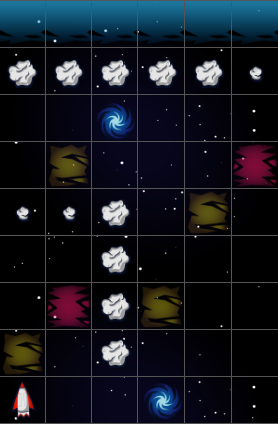
\includegraphics[width=.9\textwidth]{img/spaceworld}
%\end{subfigure}
%\begin{subfigure}{.36\textwidth}
%\centering
%{\lstset{numbers=none}
%\begin{lstlisting}
%|b |b |b |b |b |b |
%|kA|kA|kA|kA|kA|kM|
%|k |k |kW|k |k |k |
%|k |y |k |k |k |r |
%|kM|kM|kA|k |y |k |
%|k |k |kA|k |k |k |
%|k |r |kA|y |k |k |
%|y |k |kA|k |k |k |
%|kS|k |k |kW|k |k |
%\end{lstlisting}}
%\end{subfigure}
%\end{center}
%\caption{Example of Space World with its source code. TODO: Describe letters; consider replacing code listing with a screenshot from task editor with code highlighting}
%\label{fig:spaceworld-source}
%\end{figure}


\imgW[0.7]{spaceworld-in-editor}%
{Example Space World with its description. % source code.
Each line represents one row of the grid
and is split by pipes (``|'') into fields.
Each field starts with a lower-case letter denoting color of the field
(e.g. b = blue, k = black),
followed by an optional upper-case letter denoting an object
(A = asteroid, S = spaceship, etc.).
For example, ``rD'' is a red field with a diamond.}



\section{RoboCode}
\label{sec:robocode}

\emph{RoboCode} is a Python-like programming language
for representing solutions in task sources.
It closely corresponds to the text written on Blockly blocks
with a few exceptions, such as %added parentheses
shorter function names and added parentheses
(e.g. \texttt{left()} instead of \texttt{fly left}).
% also: fly right -vs- fly()
% and abbreviated literals (e.g. ``b'' instead of ``blue'').
% difference: parenthesis (color() vs. color) and literals ('b' vs. blue)
% TODO: check the statement above
It is also intended to be used in more advanced problem sets as the
transitional phase from block-based to text-based programming.
The language was designed % with the following requirements in mind:
to be simple for beginners, understandable without its previous knowledge,
concise (short, but readable programs),
and matching Python closely (for an easy transition to Python).

%\subsection{Syntax and Semantic}
%\label{sec:syntax-semantic}

% TODO[consider] note on mixing lexer+parser+some semantic analysis
% (which is partially convenient, partially confusing)

There are four basic commands: % for performing actions:
\texttt{fly()},
\texttt{left()},
\texttt{right()}, and
\texttt{shoot()}.
%\begin{lstlisting}
%fly()
%left()
%right()
%shoot()
%\end{lstlisting}
Each action is combined with moving one row forward.
The movement takes place after the action, with the exception of left and right turning actions, where the movement and the action happen simultaneously,
i.e. the spaceship flies diagonally to the left or to the right.
% TODO: Rephrase. Is confusing, because the general statement ("movement takes
% place after the action") is only relevant for shoot(), and all the other
% commands are special cases.

Loops and conditional statements are same as in Python,
with an exception of the repeat loop,
which was simplified % to a form
% matching a corresponding Blockly block, which is
to be easier to understand: % by beginners:
% TODO: ass robocode highlighting
\begin{lstlisting}
repeat 4:
    fly()
\end{lstlisting}

Conditions %inside while-loops and if-statements
are restricted to the following forms.
% (again in order to match the respective Blockly blocks):
(Color codes are same as in the Space World description,
i.e. 'r' is red, 'g' is green' etc.)
% (again in order to match the respective Blockly blocks):
\begin{lstlisting}
position() [==|!=|>|<|>=|<=] [1..6]
color() [==|!=] ['r'|'g'|'b'|'y'|'k']
<test> [and|or] <test>
\end{lstlisting}
Control structures can nest arbitrarily:
% TODO: Program for solvint the task from the previous section
%       (change either the program, the task, or both).
%\begin{figure}[h]
\begin{lstlisting}
while color() != 'b':
    if position() == 1:
        right()
    if position() >= 4:
        shoot()
    fly()
\end{lstlisting}
%\caption{Example of a complete RoboCode program}
%\label{fig:robocode-example}
%\end{figure}


\subsection{RoboAST}

While Python-like RoboCode is convenient for writing sample solutions,
a more compact form would be better for logging, storing in DB and analysis.
Secondly, a block-based presentation of the code is needed for students.
Last but not least, a JavaScript equivalent of the code is useful for
interpreting the code in the browser.
\Cref{tbl:code-representation} shows an overview of all representations.


\begin{table}[htb]
\centering
\caption{Different code representations used within the system.}
\begin{tabular}{l l l}
\toprule
Name & Form & Usage  \\
\midrule
RoboCode     & text (Python-like) & sample solutions in task sources  \\
MiniRoboCode & text (compact) & logging, storing in DB, analysis  \\
RoboBlocks   & blocks (Blockly) & code editor for students  \\
RoboJS       & text (JavaScript) & interpretation in browser  \\
RoboAST      & JSON (AST) & intermediate representation \\
\bottomrule
\end{tabular}
\label{tbl:code-representation}
\end{table}

% TODO: [consider] Use "presentation" for the "fringe" representations.
% (Because it is confusing to talk about common representation of representations.)
To avoid implementing separate transformations between each pair of these
representations, we introduced a common intermediate representation,
\emph{RoboAST}, which is an %simple
\emph{Abstract Syntax Tree} \cite{ast} in JSON
(\cref{fig:robocode-transformations-example}).
For each of the four other representations, it is enough to implement
its parser returning RoboAST object, and
its generator from RoboAST (\cref{fig:robocode-transformations}).
With a parser and a generator for each representation,
%it is possible to transform representation A
%into representation B by parsing A into RoboAST and
%then generating B from this RoboAST.
any representation A can be transformed into any representation B
by first parsing A into RoboAST and then generating B from this RoboAST.
% "This mechanism ..."
% TODO: mention the disadvantage - not able to use functionality provided by Blockly (code generators)

% TODO: fix the image (missing black line on right) (+ make it lower: tree-like
% structure, with RoboAST as a root at the top.)
\imgW[0.6]{robocode-transformations}{Transformations between RoboAST and other representations.}

\imgW{robocode-transformations-example}{Example of a RoboAST (in the middle),
  and corresponding RoboBlocks, RoboCode, MiniRoboCode, and RoboJS.}


\subsection{Parsing Expression Grammar}

For parsing RoboCode into RoboAST, we use a \emph{parsing expression grammar}
(PEG) \cite{peg}.
% TODO: verify the following statement
PEGs are essentially unambiguous context-free grammars with prioritized rules
and more compact syntax.
% and lookahead expressions (TODO: example).  % using our grammar - if we don't
% use it, then don't mention it.
% TODO: check grammar (should ... be transformed)
The PEG implementation we use%
\footnote{PEG.js, available at \url{https://pegjs.org}.}
allows to define a \emph{match result} for each parsed subexpression,
using an arbitrary JavaScript code returning a subtree of the final AST.
For illustration, there are
two % a few
examples of RoboCode parsing rules:

\begin{lstlisting}
CompoundStatement = IfStmt / WhileStmt / RepeatStmt
WhileStmt = "while" __ t:Test ":" b:Body
  { return { head: "while", test: t, body: b } }
\end{lstlisting}
%Test
%  = CompoundTest
%  / SimpleTest

PEGs can be parsed in linear time, they do not require a separate lexer,
and the resulting grammar is readable and concise;
the PEG for RoboCode % (as described in \cref{sec:syntax-semantic})
has only about 100 lines. % of code.
However, a preprocessing of the RoboCode is necessary, because
PEGs are context-free,
while RoboCode is a context-sensitive language
-- the context is created by indentation.
In addition, it is also useful to store line numbers alongside the statements
to enable \emph{meta-interpreting},
such as showing executed line, or linking errors to the point in the source code.
Therefore, the preprocessing step transforms the code in a context-free form,
in which each line of the code is prepended corresponding line number,
and adding and removing indentation levels is denoted by \texttt{\{}
and \texttt{\}} characters respectively.
For example, the preprocessed code for the program shown in
\cref{fig:robocode-transformations-example} would be:
\begin{lstlisting}
1| shoot()
2| repeat 4:
{
3| right()
4| left()
}
\end{lstlisting}
% The \cref{fig:robocode-transformations-example} also shows the final RoboAST object.

\subsection{MiniRoboCode}
\label{sec:minirobocode}

MiniRoboCode is a condensed form of the RoboCode.
It replaces indentation by curly brackets,
keywords and functions by their first letters,
and removes whitespace characters
in order to fit programs into a single short line.
The mapping from the RoboCode is described by the following rules:
% shown in \cref{fig:minirobocode-transformation-rules}.
\smallskip

\noindent\begin{minipage}{.49\textwidth}
\begin{lstlisting}[numbers=none]
repeat --> R
while --> W
if --> I
else --> /
position() --> x
== --> =
\end{lstlisting}
\end{minipage}\hfill
\begin{minipage}{.49\textwidth}
\begin{lstlisting}[numbers=none]
fly() --> f
left() --> l
right() --> r
shoot() --> s
color == 'y' --> y
color != 'y' --> !y
\end{lstlisting}
\end{minipage}

%\begin{figure}[h]
%\begin{subfigure}{.49\textwidth}
%{\lstset{numbers=none}
%\begin{lstlisting}
%repeat --> R
%while --> W
%if --> I
%else --> /
%position() --> x
%== --> =
%\end{lstlisting}}
%\end{subfigure}
%\begin{subfigure}{.49\textwidth}
%{\lstset{numbers=none}
%\begin{lstlisting}
%fly() --> f
%left() --> l
%right() --> r
%shoot() --> s
%color == 'y' --> y
%color != 'y' --> !y
%\end{lstlisting}}
%\end{subfigure}
%%\caption{Transformation rules from RoboCode to MiniRoboCode. (In reality, the transformations goes through RoboAST.)}
%%\label{fig:minirobocode-transformation-rules}
%\end{figure}
% \Cref{fig:minirobocode-transformations} shows
\smallskip

\noindent
Two examples of complete transformations into MiniRoboCode:
\smallskip

\noindent\begin{minipage}{.49\textwidth}
\begin{lstlisting}[numbers=none]
fly()
while color() == 'b':
    left()
    right()
fly()
<*\arrowlinesplit*>
fWb{lr}f
\end{lstlisting}
\end{minipage}\hfill
\begin{minipage}{.49\textwidth}
\begin{lstlisting}[numbers=none]
repeat 6:
    if position() > 1:
        shoot()
    else:
        right()
<*\arrowlinesplit*>
R6{Ix>1{s}/{r}}
\end{lstlisting}
\end{minipage}
\smallskip

%\begin{figure}[h]
%\begin{subfigure}{.49\textwidth}
%{\lstset{numbers=none}
%\begin{lstlisting}
%fly()
%while color() == 'b':
%    left()
%    right()
%fly()
%-------------------
%fWb{lr}f
%\end{lstlisting}}
%\end{subfigure}
%\begin{subfigure}{.49\textwidth}
%{\lstset{numbers=none}
%\begin{lstlisting}
%repeat 6:
%    if position() > 1:
%        shoot()
%    else:
%        right()
%-------------------
%R6{Ix>1{s}/{r}}
%\end{lstlisting}}
%\end{subfigure}
%%\caption{Examples of transformations of RoboCode to MiniRoboCode.}
%%\label{fig:minirobocode-transformations}
%\end{figure}

MiniRoboCode is useful not only for logging and storing programs in the database,
but also for many analyses, because it is easy to process by counting
letters or matching simple regular expressions, and because they are short
enough to be used as labels in plots.


\subsection{RoboBlocks}

Blockly%
\footnote{Available at \url{https://developers.google.com/blockly/}.}
is an implementation of block-based programming
environment from Google,
which we use in the code editor for students
(shown e.g. in \cref{fig:robomission-task1}).
% TODO: ref to section about block-base programming envs and their pros/cons
% TODO: mention advnatages of using Blockly from Google: well-tested, widely-used
% (and disadvantage: don't play nicely with modern JS workflow; sometimes needs
% awful hacks to digging in the source code to achieve a desiered behavior
Blockly allows to import and export the currently assembled program in
an XML format, that we call \emph{RoboBlocksXML}
%(See \cref{fig:roboblocks-xml} for an example of the XML.)
(\cref{fig:roboblocks-xml}).
Both transformations between RoboBlocksXML and RoboAST are straightforward.

% TODO(opt): some details about Blocly? (definition of blocks)
%  (or just overview of currently used blocks (in a row "toolbox" to save space)

% TODO: make it just refferable listing, instead of figure
\begin{figure}[h]
\begin{lstlisting}[basicstyle=\small\ttfamily]
<xml xmlns="http://www.w3.org/1999/xhtml">
 <block type="start">
  <next><block type="shoot">
   <next><block type="repeat">
    <field name="count">4</field>
    <statement name="body">
     <block type="fly">
      <field name="direction">right</field>
      <next><block type="fly">
       <field name="direction">left</field>
      </block></next>
     </block>
    </statement>
   </block></next>
  </block></next>
 </block>
</xml>
\end{lstlisting}
  \caption{%
    RoboBlocksXML for the program shown in %
    \cref{fig:robocode-transformations-example}.}
\label{fig:roboblocks-xml}
\end{figure}

As the RoboBlocks are used by children, it is important to use localized labels
on the blocks.
Depending on the language domain, we initialize Blockly blocks with the corresponding
version of localized block labels
(\cref{fig:roboblocks-english-czech}).
%(See \cref{fig:roboblocks-english-czech} for an example of the same program in two languages.)
%Blockly supports its own localization mechanism that fits well
%within the localization framework used in our project.

\imgW[0.5]{roboblocks-english-czech}{Same program in English and Czech localizations of RoboBlocks.}
% TODO: Fix the image so that both images are of the exactly same size and sharpness.

\subsection{RoboJS and Interpretation}
\label{sec:robomission-robojs}

Instead of implementing our own interpreter of RoboCode,
we transform the code through RoboAST into JavaScript,
%(described in \cref{sec:robomission-robojs})
and then use a JavaScript interpreter to run the code.
The generated \emph{RoboJS} % is just a JavaScript that
assumes to be executed within a
context providing hooks for functions corresponding to actions (\texttt{fly}, \texttt{left}, \texttt{right}, \texttt{shoot}),
sensors (\texttt{color}, \texttt{position}),
and meta-interpreting (\texttt{isStopped}, \texttt{highlightBlock})
(\cref{fig:robojs-example}).

The interpreter does not have to be necessary a \emph{JavaScript} interpreter,
since it is easy to transform RoboAST to any other common imperative language.
% (at least to the common imperative languages).
However, the interpreter must satisfy the following requirements:
% TODO: check grammar: "to be implemented ... to allow ..."?
be implemented in JavaScript (to run in the browser),
allow to define custom asynchronous hooks
(to perform actions),
%(in order to perform actions, sensor measurements, and block highligting),
and allow to step the code, or at least to impose a limit on
the number of steps % or time
(to break infinite loops).
%(in order to break infinite loops).
% interprets a language that can be generated easily from the RoboAST (which includes most languages),
%There is nothing special about using JavaScript as the language being interpreted,
%other that the JS-interpreter satisfies all our requirements
%and is relatively simple to use.

% We could use any interpreter that would satisfy the following conditions:
%\begin{enumerate}
%\item is implemented in JavaScript (in order to run in the browser),
%\item interprets a language that can be generated easily from the RoboAST
%  (which includes most languages),
%\item allows to define custom asynchronous hooks
%  (needed for actions, sensors, and block highligting),
%\item allows to step the code, or at least to impose a step or time limit
%  (in order to break infinite loops).
%\end{enumerate}
% TODO(opt): why not to use JS interpreter in browser: safety (sandbox requirement)
% + probably also not able to step the code or set the time limit, but I haven't verified this


%For the interpretation of the student code yet another representation is needed,
%a JavaScipt code that can be fed into a JS interpreter.
%(See \cref{sec:robomission-interpretation} for the details of the interpretation).


\begin{figure}[h]
\begin{subfigure}{.28\textwidth}
\centering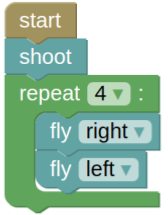
\includegraphics[width=.8\textwidth]{img/roboblocks-english}
\end{subfigure}
\begin{subfigure}{.7\textwidth}
{\lstset{numbers=none}
\begin{lstlisting}
highlightBlock(1);
shoot();
highlightBlock(2);
for (var i1_ = 0; i1_ < 4; i1_++) {
  highlightBlock(3);
  right();
  highlightBlock(4);
  left();
}
\end{lstlisting}}
\end{subfigure}
\caption{%
  Example of a RoboJS (right) for given RoboBlocks program (left). %
  % Repeat loops require to generate unique names for iteration variables.
  Each original command is accompanied by \texttt{highlightBlock(blockId)},
  so that the meta-interpreter knows which block to highlight.}
\label{fig:robojs-example}
\end{figure}

%We have not implemented a parser from RoboJS to RoboAST,
%simply because we do not need this tranformation;
%otherwise, there is no technical obstacle and the parser would be based on a similar PEG gramamar as for the RoboCode.

We use an existing JavaScript interpreter%
\footnote{JS-interpreter, available at \url{https://github.com/NeilFraser/JS-Interpreter}.}
and wrap it into two
additional layers: the first layer is a generator
that yields actions, sensor requests and
meta-interpreting effects (e.g. block highlighting), % checking for interruption).
and the second layer is a saga
%(see \cref{sec:robomission-asynchronous-side-effects})
that handles all these asynchronous effects.
The separation into these two layers allows to test the interpreter logic
easily without dealing with asynchronous effects.

\chapter{Analysis of Collected Data}
\label{chap:analysis}

In order to get insight into how the deployed system works
and what should we focus on in next iterations,
we analyze collected data.
All analyses in this chapter use data collected  % avoid repeating "collected"
during 4 months (10th November 2017 -- 9th March 2018).
This data, as well the code performing the analyses, are available
as attachments of this thesis
(described in \cref{sec:attachment.collected-data,sec:attachment.analyses}).


\section{Data Description}

During the 4 months, about 1000 users tackled at least one task,
%\footnote{The true number of unique users might be lower, because a single user
%may be counted multiple times if he had not signed up and used the system again
%after a session cookie had expired. However, the Google Analytics suggests
%that the number is approximately correct.},
and 800 of them solved at least one task.
About 100 students returned and solved another task another day.
\Cref{fig:engagement-curves} shows complete engagement curves.
% TODO (GA):
Nearly all users access the webpage on a desktop computer ($94\%$).
% TODO: and does any of the mobile-users solved any task? (because that would be very difficult)
% Desktop 94%, Mobile 4%, Tablet 2%

\begin{figure}[htb]
\centering
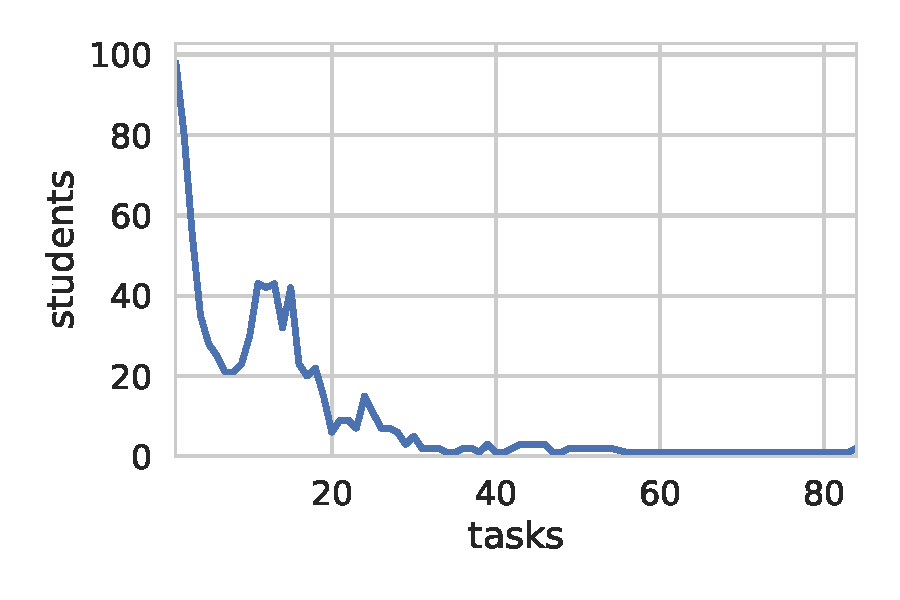
\includegraphics[width=0.48\textwidth]{img/engagement-tasks}
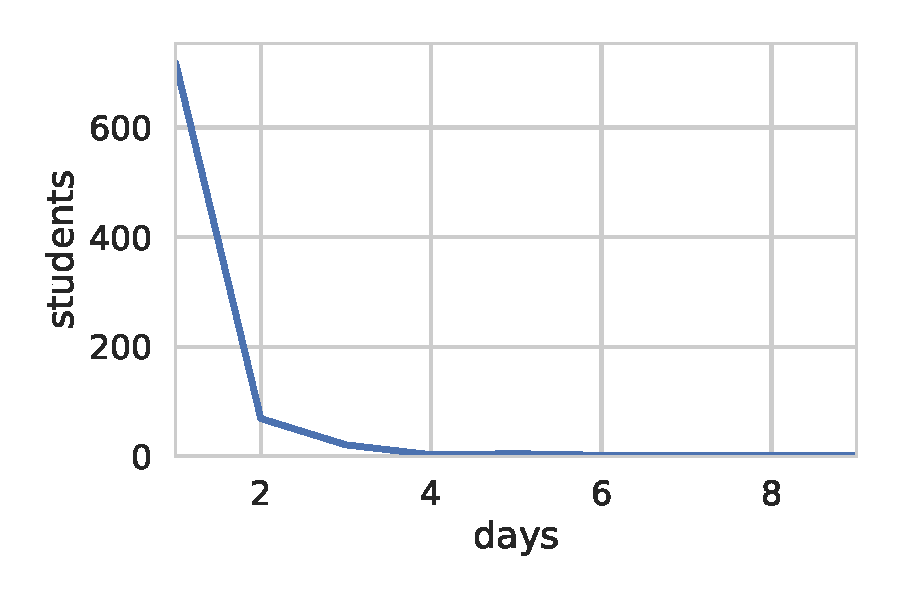
\includegraphics[width=0.48\textwidth]{img/engagement-days}
\caption{%
  Engagement curves.
  Left: How many students solved given number of tasks.
  Right: How many students solved a task given number of days.}
\label{fig:engagement-curves}
\end{figure}


About 11000 tasks were attempted (counting only those with at least one edit),
and 9600 of them were solved,
resulting in the overall success rate $86\%$.
The daily numbers of solved task sessions are not stable,
with high peaks on days when the application was used
in a competition or testing at a school
(\cref{fig:daily-task-sessions}).
% The following can be a separate paragraph, if another
% analysis is performed.
Over 180 thousand program snapshots was collected,
from which 140 thousand corresponds to edits,
and 40 thousand to executions.

% TODO: join with another plot (-> two plots on a single line).
% (e.g. a metric mentioned at the theory part)
% TODO: crop/tighten margings (esp. the bottom one)
%\imgW[0.3]{daily-task-sessions}{%
%  Daily number of solved task sessions (weekly averaged).}
\begin{figure}[htb]
\centering
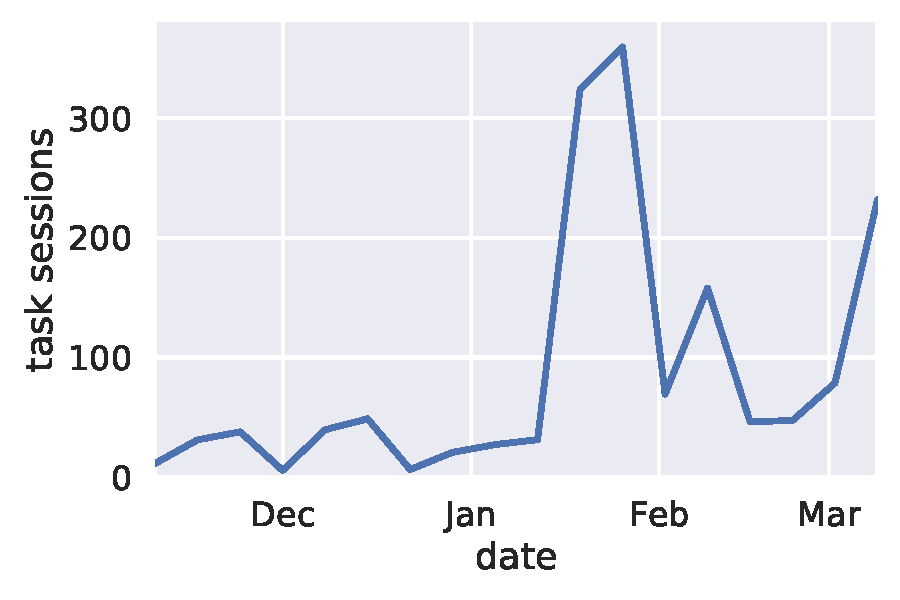
\includegraphics[width=0.48\textwidth,trim={0 21mm 0 7mm},clip]{img/daily-task-sessions}
\caption{Daily number of solved task sessions (weekly averaged).}
\label{fig:daily-task-sessions}
\end{figure}

Median solving time is 60 seconds (interquartile range: 24-145 seconds).
Solving times follow log-normal distribution (\cref{fig:solving-times}),
so the mean solving time is much higher (even if the times are capped at one hour):
195 seconds, with high standard deviation of nearly 500 seconds.


\begin{figure}[htb]
\centering
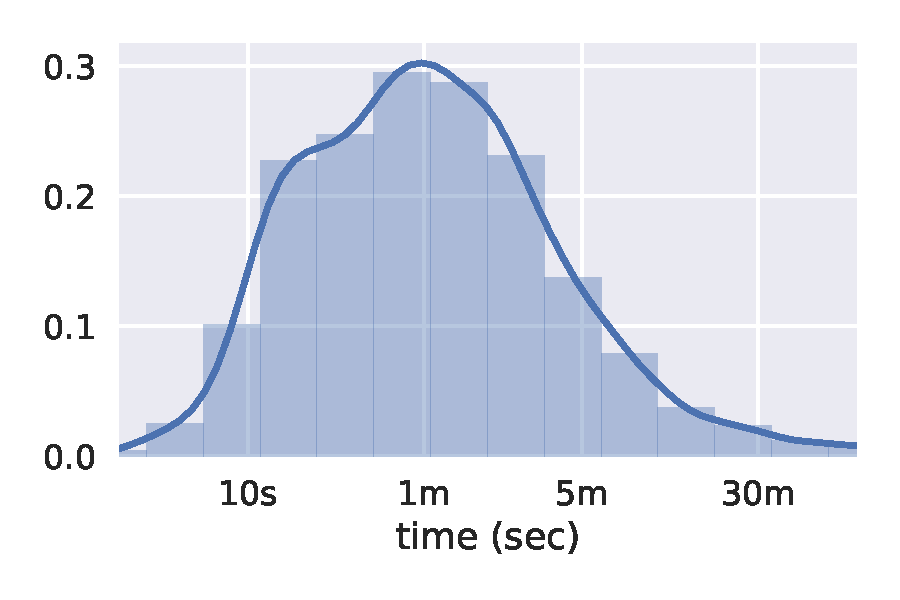
\includegraphics[width=0.48\textwidth]{img/task-sessions-time-log}
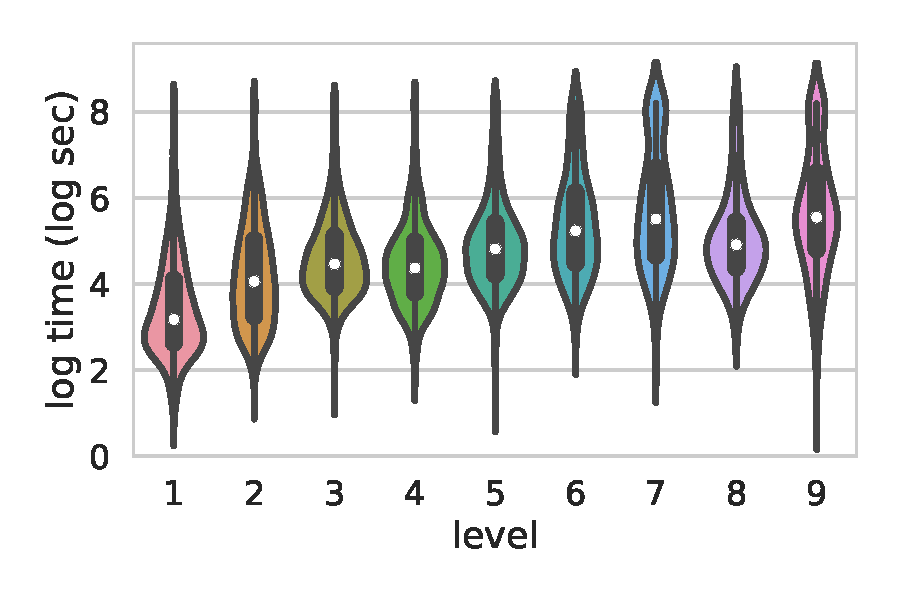
\includegraphics[width=0.48\textwidth]{img/levels-time}
\caption{%
  Distribution of log-transformed solving times.
  Left: All task sessions.
  Right: For each level.}
\label{fig:solving-times}
\end{figure}

\section{Performance Compression}

% In ... we have discussed importance of a performance compression
Our student model uses three-valued performance representation, and
a performance compression function based purely on observed solving time
(\cref{sec:robomission.student}).
Would using other observational data, such as number of edits
bring more information about the performance?
(TODO: Goal: find a compression function that maximizes performance of
student model.)

Overall Pearson correlation between solving times and number of edits (both
log-transformed) is quite high (0.73). However, if computed for individual tasks,
median correlation drops to 0.64, % (interquartile range 0.5 -- 0.72),
and $25\%$ of tasks have a correlation below 0.5 % check the number
(\cref{fig:time-vs-edits}), which suggests that incorporating number of edits
(or executions) should be at least considered.


\begin{figure}[htb]
\centering
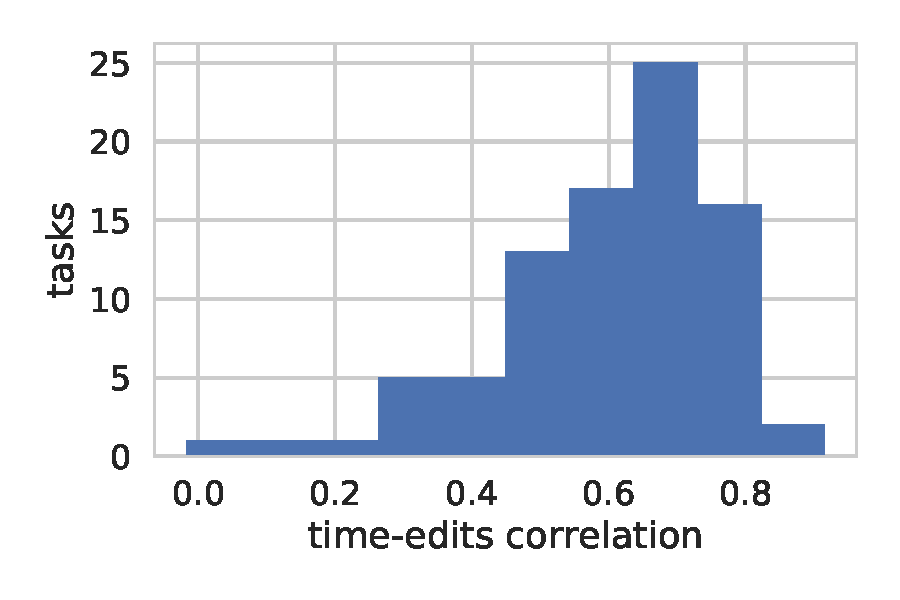
\includegraphics[width=0.48\textwidth]{img/time-edits-corr}
%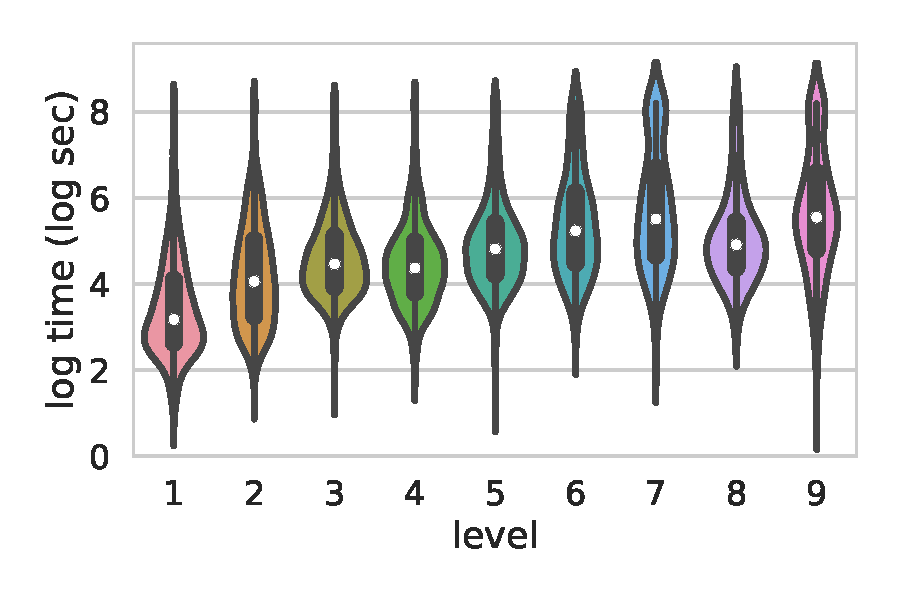
\includegraphics[width=0.48\textwidth]{img/levels-time}
\caption{%
  Distribution of Pearson correlations between median solving times and number
  of edits (both log-transformed) for individual tasks.} %  TODO: another plot on the right.}
\label{fig:time-vs-edits}
\end{figure}


\section{Task Difficulties}

% TODO: Resolve mission vs. level.
Our tutor model (\cref{robomission.tutor}) assumes that difficulties of tasks
in a phase are approximately same,
and that the overall difficulty is increasing as the level increases.   % even phase.
Using collected data, we can determine whether these assumption are satisifed,
and if not, suggest adjustments to improve their validity.

\Cref{fig:solving-times} (right) shows that on average the difficulty of levels
is increasing, but it also reveals that level 7 is more difficult than level 8.
% TODO: Elaborate on the solution to this issue.
% (TODO?: phases instead of missions, and select only a few to save space)
Looking at the difficulty of individual tasks (\cref{fig:difficulties-tasks-levels})
help us to discover outliers, whose difficulty is significantly
different from the other tasks in the same level.
The \cref{fig:difficulties-tasks-levels} also suggests that dividing levels
into phases is necessary to achieve reasonable homogenity. For example, in the 2nd
level (World), there are two clear groups of tasks with significantly different
difficulty. Although in the other levels such a clear split does not exist,
they still often contain tasks with a wide range of difficulties.
% TODO: note/analyze robustness of these analyses (given the limited data)

% TODO: only a first 6 levels or possibly devide into phases
\begin{figure}[htb]
\centering
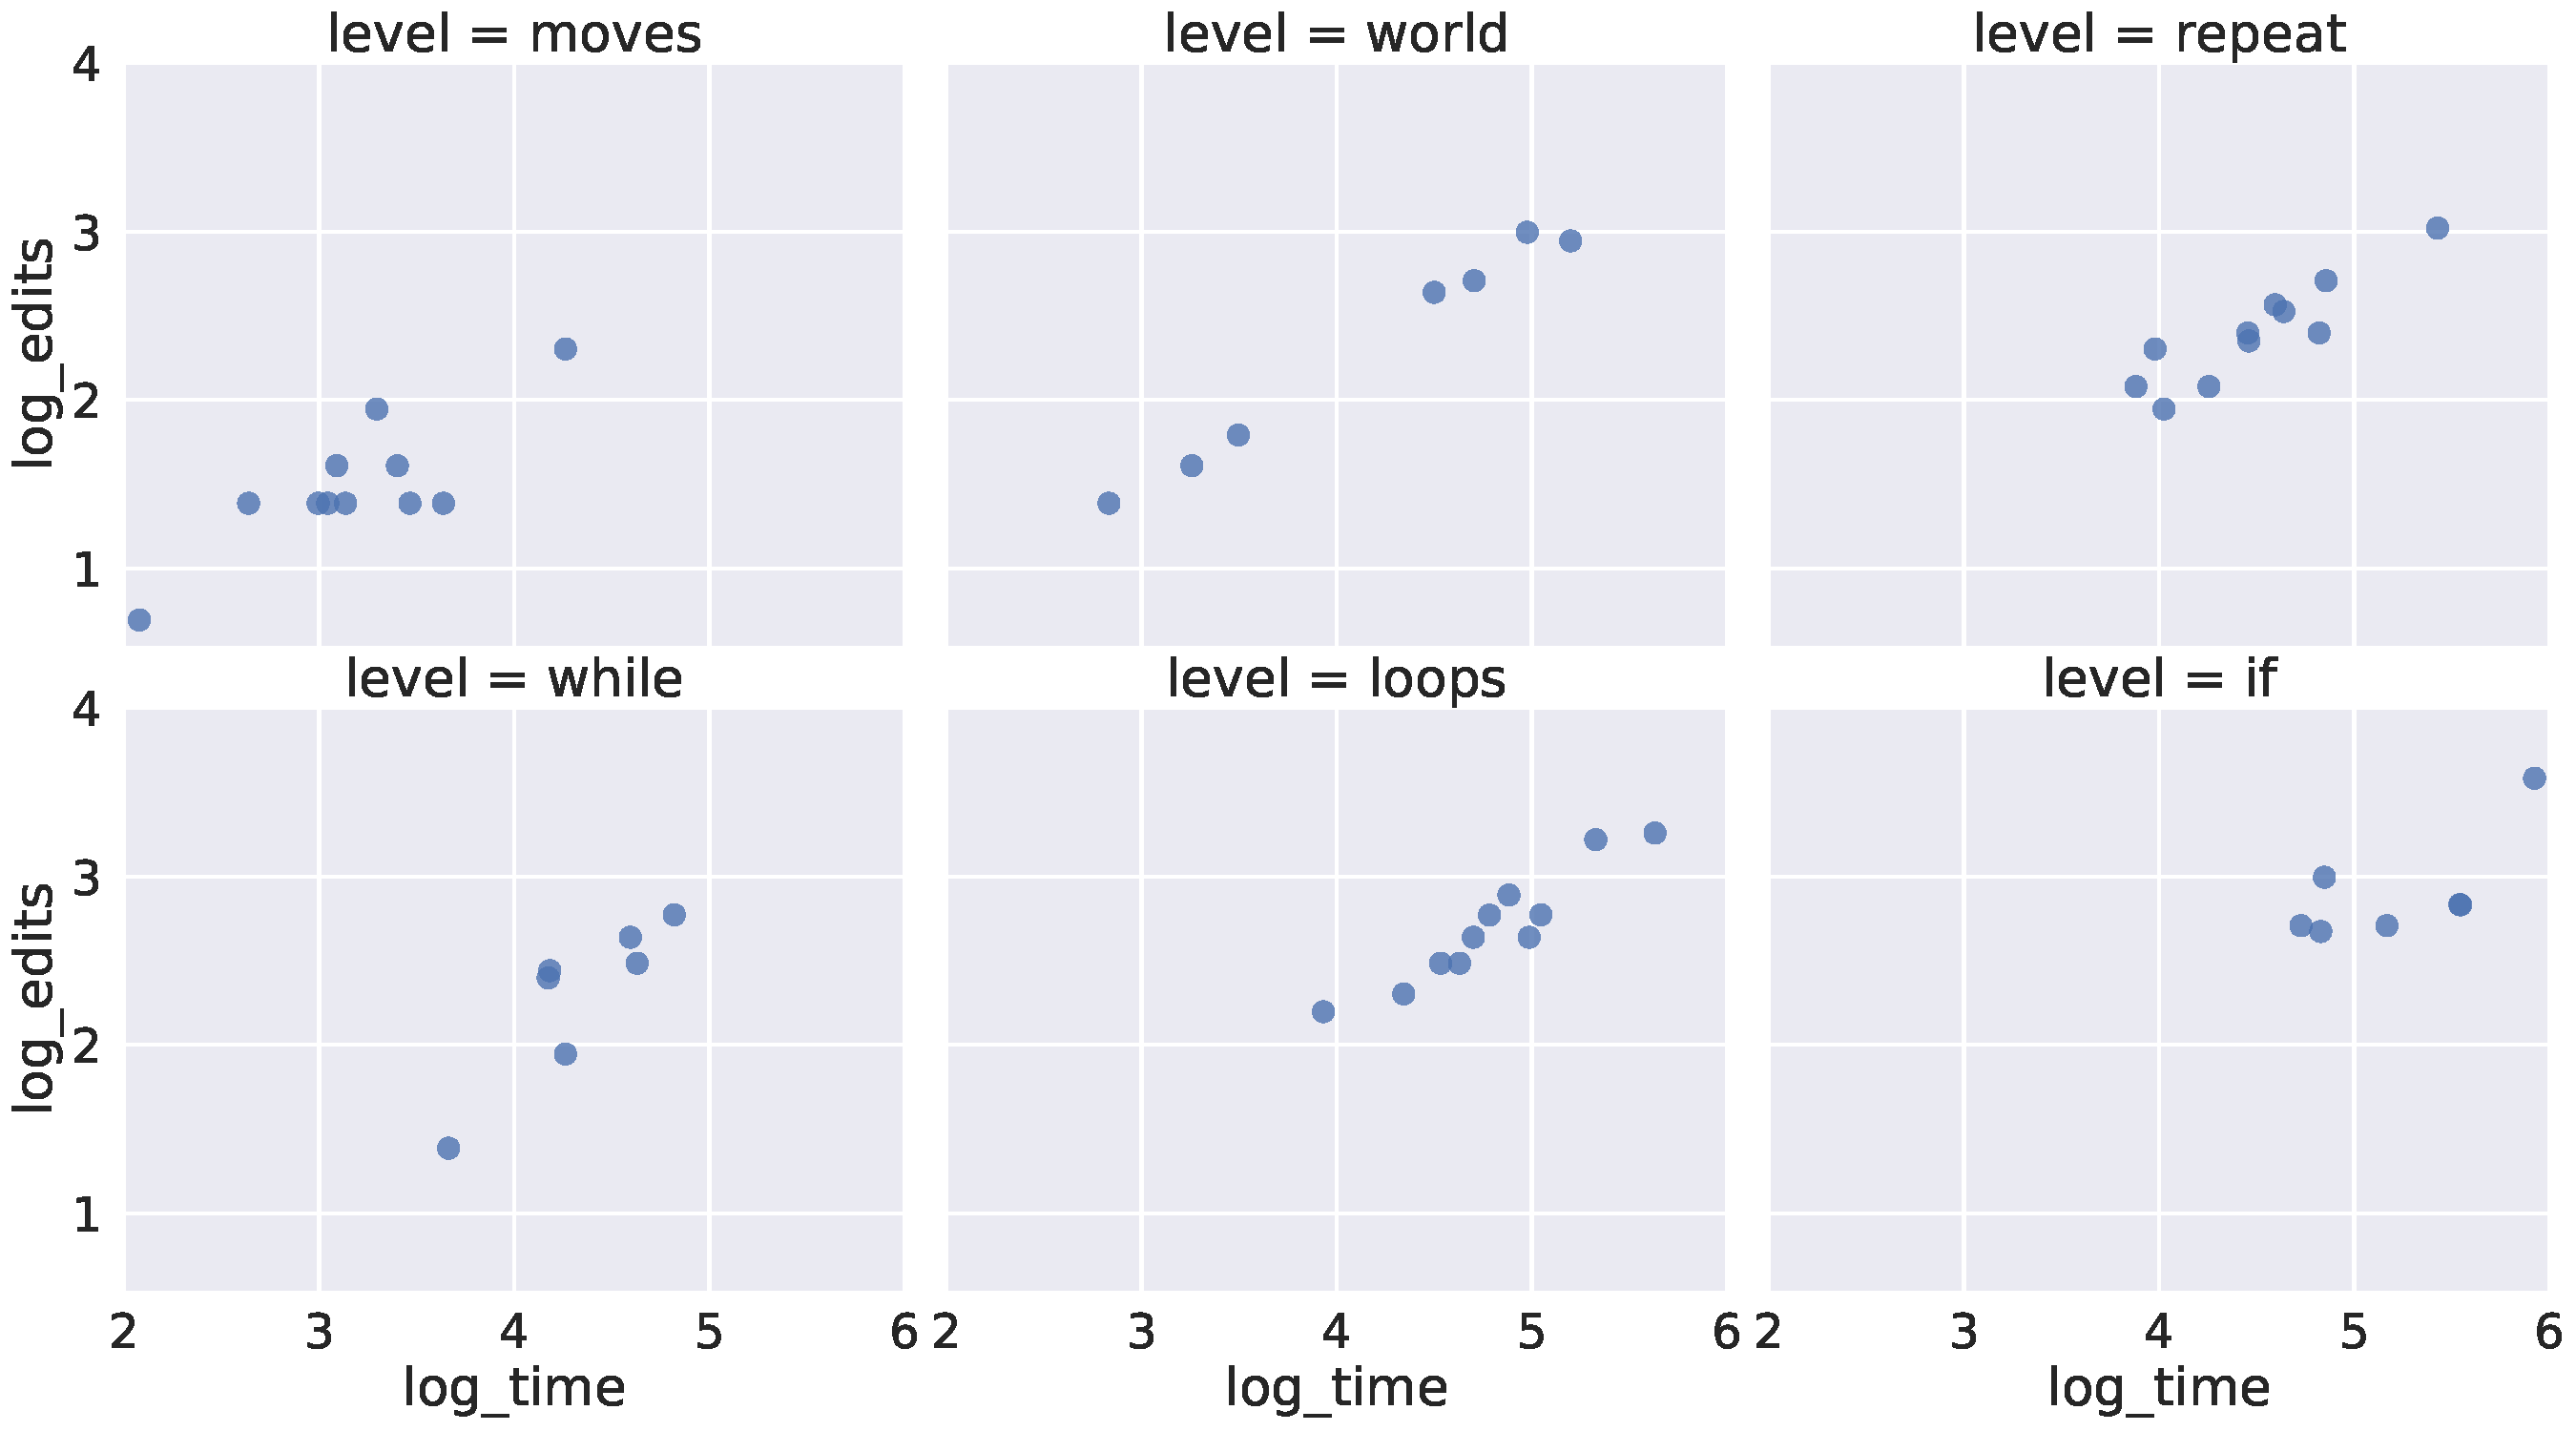
\includegraphics[width=\textwidth]{img/difficulties-tasks-levels}
\caption{%
  Difficulties of tasks in first 6 levels.
  Difficulty is measured as spent time and number of edits, both log-transformed.}
\label{fig:difficulties-tasks-levels}
\end{figure}

%\imgW{difficulties-tasks-levels}{%
%  Difficulties (spent times and number of edits, both log-transformed)
%  of tasks in each level.}

\chapter{Conclusion}
\label{chap:conclusion}

\itquote[0mm]{
Shoot for the moon. Even if you miss, you'll land among the stars.
}{B. Littrell}

%\section{Summary}
%\label{sec:conclusion.summary}

This thesis describes how a combination of several strategies to support
learning and motivation, together with the adaptivity of the system
through techniques of artificial intelligence,
can lead to efficient learning of introductory programming. % too strong?
Creating such a system is, however, not a one-shot task, but rather a long series
of small iterative improvements of a programming game,
models of the domain, student and tutor, user interface, and the analysis layer.

With our adaptive system for learning programming, RoboMission,
we have already completed a few iterations of improvements.
% our adaptive learning system for introductory programming,
Since its first prototype, which was implemented in 2015,
%we use the feedback from users (as well as collected data?)
we have completely changed both the programming game and the adaptive behavior.
The version deployed in November 2017 was used during the following four months
by about 1000 users, who solved about 10000 tasks.
We tested its usability at schools during Hours of Code,
as well as in two competitions for primary and secondary school students,
Purkiáda\footnote{\url{http://purkiada.sspbrno.cz}} and
InterSoB\footnote{\url{https://intersob.math.muni.cz/2018/}}.
% (Purkiada, Sob 2018) Sob - consider including a photo
We have published  our initial research on programming tasks similarities \cite{alg.similarity}
and on the adaptive approach to learning programming \cite{robomission}.

% \imgW[0.7]{intersob}{InterSoB ... (Photo by Vendula Němcová.}

% \section{Lessons Learned}

%\section{Future Work}
%\label{sec:conclusion.future-work}

Many improvement iterations are yet to be undertaken. After adding
new game elements and programming concepts (e.g., functions and compound
conditions), it will be possible to create more advanced problem sets
and extend the use case of the system beyond the short motivational tutorial.
% (\emph{Hour of Code mode}).  % grammar
Tasks could gradually transition from block-based to Python programming
and teach even advanced algorithmic concepts (\cref{fig:robomission-search-tree}).
Next, we plan to implement a real-time dashboard for teachers,
which would visualize the progress %and skills
of students and suggest
which students need help right now, and possibly even how to pair students
for efficient pair programming.

% EXT:
% ... (\emph{Hour of Code mode}).
%In \emph{foundations mode}, students could spend from a few days to several weeks practicing
%programming, transitioning gradually from block-based to textual programming
%in RoboCode.
%% missions for learning new programming elements, esp. functions and compound conditions
%% Usage: for a standard primary-secondary school programming curriculum.
%Then, in \emph{university mode} targeting at high school and university students,
%tasks would teach programming in Python, and possibly even advanced algorithmic
%concepts (\cref{fig:robomission-search-tree}).
%% at home / secondary schools, KSI (0th problem set), IB111 (0th/1st motivational lesson)
%Furthermore, we would like to introduce a \emph{competition mode}, for
%straightforward usage of new tasks in a programming contest,
%leaving these problem sets public for everybody for practice once the
%competition is over.
% Competitions --  (both blocks and Python depending on the competition) such as Purkiada, Pevnost FI, KSI, InterLos, InterSob, new FIBot (new problem sets -> public for everybody for practice after the competition; %this also includes testing mode for RH interns
% 5. Cooperation: multiplayer programming game

\begin{figure}[htb]
\centering
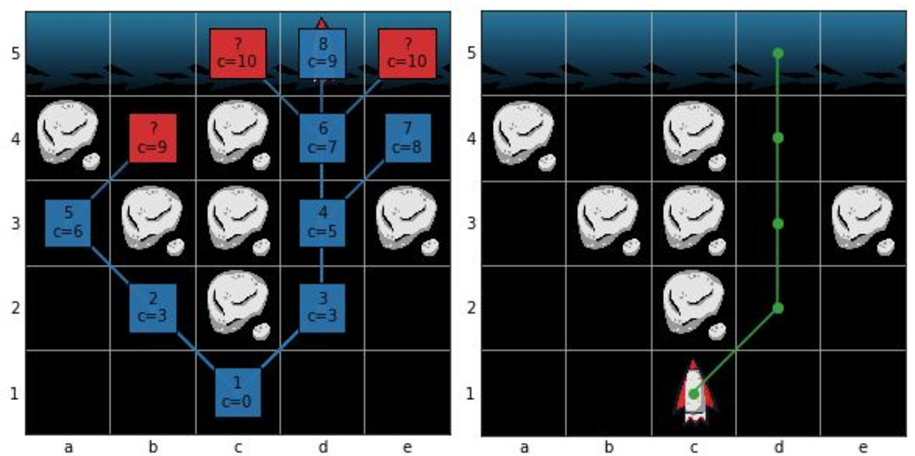
\includegraphics[width=\textwidth]{img/robomission-search-tree}
\caption{%
  Example of how the Space World can be used for learning algorithms,
  in this case Dijkstra's shortest path algorithm
  (used at a workshop for high school students).}
\label{fig:robomission-search-tree}
\end{figure}


With growing content, it would become useful to build more complex
domain, student and tutor models. In order to add overlapping concepts
into the domain and use them to predict student performance more accurately,
we need to analyze how multiple skills interact in a single
task to produce the final performance. %, in order to predict performance.
% in a single task. % to produce a single performance.
Using data from a single task session,
we want to detect which concepts contained in the task
is the student struggling with.
Models might be further improved by including uncertainty of estimates,
forgetting of skills, and planning of tutor actions.

To evaluate which versions of models improve learning and motivation, %increase the learquality of the system,
analysis layer should be extended to allow for AB experiments
% In addition to compare several versions of student or tutor models,
% ... experiment on block-based vs text-based programming
and a careful attention should be paid to both long-term and
online attributable metrics.
We need to make sure that we collect enough data for reliable unbiased evaluation,
which is complicated by feedback loops caused by the fact that
the collected data which the system is evaluated on are influenced by the
adaptive behavior of the system itself.
% and long-term metrics monitoring, simulated experiments
In order to further align measured metrics with the system mission,
we can explore how to reduce noise in flow observations
by combining subjective user feedback with objective performance measures.
Having reliable flow observations would be a great step towards optimizing
the total amount of time spent in the state of flow.

%- peer tutoring (in a classroom)
% - if RL approaches can help


\printbibliography[heading=bibintoc]

\appendix

\chapter{Attachments}
\label{chap:attachments}

Source code, exported data and performed analyses
are available as attachments in the \emph{Archive of Thesis}%
\footnote{\url{https://is.muni.cz/th/410350/fi\_m/}}
in the Information System of Masaryk University,
and also in GitHub repositories of the project and the thesis.

\section{Source Code}
\label{sec:attachment.source-code}

Snapshot of the source code
(including setup instructions in \texttt{README.md})
% documentation (\texttt{docs}),
%and domain data (\texttt{backend/domain}),
is attached as \texttt{code.zip}.
The most recent version of the project is available at
\url{https://github.com/adaptive-learning/robomission}.

\section{Exported Data}
\label{sec:attachment.collected-data}

Both the domain and collected data used for analyses in this
thesis (exported on 9th March 2018) are attached as
\texttt{data.zip}, and they are also available at
\url{https://github.com/effa/flocs-thesis/tree/master/data}.
Data is exported as a few CSV tables,
with the columns described below.
%Columns of the CSV tables are described in
%\cref{tbl:data.tasks,tbl:data.levels,tbl:data.task-sessions,tbl:data.program-snapshots}.

\subsection{Tasks}

\begin{tabular}{l l}
\toprule
Attribute & Description \\
\midrule
id & ID of the task \\
name & text label of the task \\
level & name of the mission \\
setting & JSON with "fields" and optional limits ("length", "energy") \\
solution & MiniRoboCode representation of the solution (\cref{sec:minirobocode}) \\
\bottomrule
\end{tabular}

% TODO: consider to update to the new data export with PS (of course not only
% description, but also the actual export and analyses)

\subsection{Problem Sets}

\begin{tabular}{l l}
\toprule
Attribute & Description \\
\midrule
id & ID of the problem set \\
level & order of the problem set (by difficulty) \\
name & text label of the problem set \\
toolbox & name of the available toolbox \\
tasks & list of task names contained in the problem set \\
\bottomrule
\end{tabular}

\subsection{Task Sessions}

\begin{tabular}{l l}
\toprule
Attribute & Description \\
\midrule
id & ID of the task session \\
student & ID of the student \\
task & ID of the task \\
solved & whether the student solved the task (boolean) \\
start & timestamp of opening the task \\
end & timestamp of the last action in the task session \\
time\_spent & length of the task session in seconds \\
\bottomrule
\end{tabular}


\subsection{Program Snapshots}

\begin{tabular}{l l}
\toprule
Attribute & Description \\
\midrule
id & ID of the program snapshot \\
task\_session & ID of the task session \\
time & timestamp of creating the snapshot \\
program & MiniRoboCode representation of the code (\cref{sec:minirobocode}) \\
granularity & "edit" or "execution" \\
order & order of the snapshot of this granularity in the session \\
correct & whether the execution was successful (empty for edits) \\
time\_from\_start & seconds from the start of the task session \\
time\_delta & seconds from the previous snapshot of same granularity \\
\bottomrule
\end{tabular}


\section{Analyses}
\label{sec:attachment.analyses}

The last attachment (\texttt{analysis.zip})
contains several Jupyter Notebooks and Python modules with the analyses
presented in the thesis.
Also available at
\url{https://github.com/effa/flocs-thesis/tree/master/analysis}.

\chapter{Used Technologies}
\label{chap:technologies}

Technolgoies used in the project change quite quickly in order to meet new requirements,
especially on frontend, where the tools and best practices are evolving rapidly.
The following tables show the overview of technologies used in the project in spring 2018.

%When this project started in 2015,
%we used several at that time popular technologies
%(AngularJS, Bootstrap, bower, grunt)
%which became obsolete during next 2 years,
%so we replaced them by newer ones.
%Many technologies were introduced naturally as the projects grew,
%e.g. Django Rest Framework for REST API,
%or redux-saga for cleaner handling of asynchronous side-effects
%(instead of the originally used redux-thunk).

\begin{table}[htb]
\centering
\caption{Project Management.}
\begin{tabular}{l l l}
\toprule
Area & Technology & Main Reason  \\
\midrule
Version control & git, GitHub & features \\
% Online repository & GitHub & easy to use \\
Custom commands & make, django, npm & easy to use \\
Monitoring & Google Analytics & easy to use \\
\bottomrule
\end{tabular}
\end{table}

\begin{table}[htb]
\centering
\caption{Backend.}
\begin{tabular}{l l l}
\toprule
Area & Technology & Main Reason  \\
\midrule
Language & Python 3 & concise, high-level \\
Dependencies & pip & standard tool, easy to use \\
Environment & virtualenvwrapper & easy to use \\
Unit tests & pytest & concise, readable \\
Web framework & Django & features, well-documented \\
REST API & DRF & features, well-documented \\
Database & PostgreSQL & widely used \\
Web server & Nginx, Gunicorn & widely used \\
Scheduled jobs & cron, django-crontab & standard tool \\
Data export & Django Rest Pandas & DataFrame tranformations \\ % before export \\
\bottomrule
\end{tabular}
\end{table}

\begin{table}[htb]
\centering
\caption{Frontend.}
\begin{tabular}{l l l}
\toprule
Area & Technology & Main Reason  \\
\midrule
Language & ES6 & concise, readable \\
Dependencies & npm & easy to use \\
Bundling & webpack & feature-complete \\ %, widely used \\
Compiling & babel & feature-complete \\ % , widely used \\
State & redux  & predictability, testability \\  % behavior, testability \\
Side effects & redux-sagas  & readability, testability \\
Views & React & declarative, reausable \\
Design (UI) & Material-UI & good appearence \\
HTTP client & axios & Promises API\\
Code blocks & Blockly & well-tested \\
Parsing & PEG JS & declarative rules \\  %(Parsing expression grammar) \\
Interpretation & JS-interpreter & stepping, custom hooks \\
Localization & react-intl & one place for all messages \\
\bottomrule
\end{tabular}
\end{table}

\begin{table}[htb]
\centering
\caption{Analysis.}
\begin{tabular}{l l l}
\toprule
Area & Technology & Main Reason  \\
\midrule
Language & Python 3 & concise, high-level \\
Documents & Jupyter Notebook & interactivity \\
DataFrames & pandas & features, well-documented \\
Plotting & matplotlib, seaborn & features, nice plots \\
%Machine learning & sklearn & powerful \\
\bottomrule
\end{tabular}
\end{table}


\end{document}
